\documentclass[11pt,a4paper]{article}

\usepackage{polski}
\usepackage{pdfpages}
\usepackage[utf8]{inputenc}
\usepackage{multirow}
\usepackage{pgf}
\usepackage{minted}
\usepackage{float}

\begin{document}

%zmienne
\newcommand{\ltabname}{Masa ciężarków[g]}
\newcommand{\rtabname}{Wydłużenie[cm]}
\newcommand{\rrtabname}{Czas wykonania 20 wahań[s]}
\newcommand{\Ts}{T[s]}
\newcommand{\pgfmath}[1]{\pgfmathparse{#1}\pgfmathresult}
% strona tytułowa sprawozdania
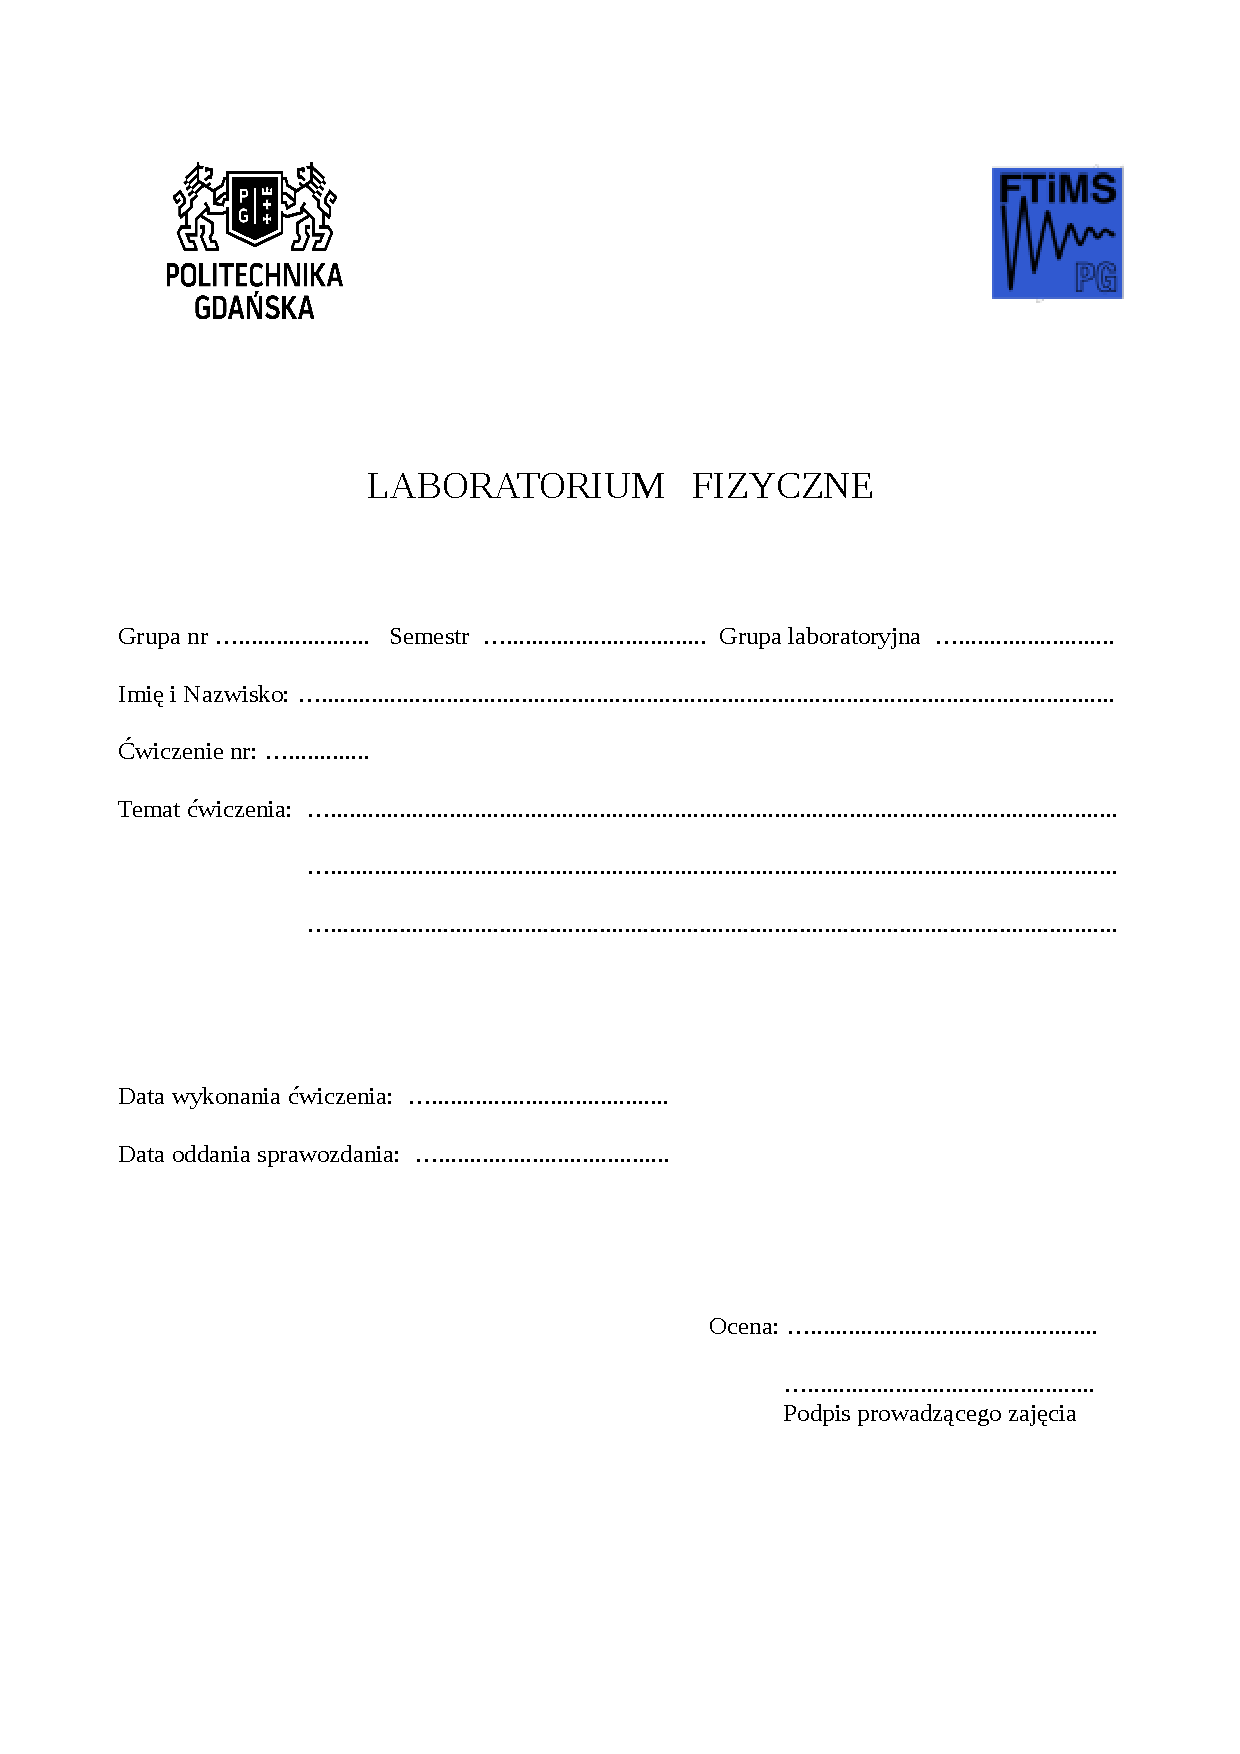
\includepdf{str_tyt.pdf}

% wstęp
    \section{Wstęp}
    Zajęcia laboratoryjne polegały na analizie ruchu drgającego ciężarka zawieszonego na sprężynie bądź układzie sprężyn, czyli pomiarze okresu drgania. Pomiary miały być dokonane dwoma metodami - statyczną i dynamiczną. Celem tego miało być wyznaczenie współczynnika sprężystości tych sprężyn oraz ich układów, a także wyznaczenie modułu sztywności materiału sprężyny.

    
    \section{Otrzymane wyniki}
    Wyniki otrzymane podczas pomiaru na laboratorium \\
    
    %pierwsza sprężyna
    \begin{center}
        Pierwsza sprężyna
        \begin{tabular}{cc}
            \begin{tabular}{ |c|c| }
                \hline
                \multicolumn{2}{|c|}{Metoda statyczna} \\
                \hline
                \ltabname & \rtabname \\
                \hline
                0 & 0 \\ 
                \hline
                50.320 & 5 \\  
                \hline
                100.342 & 10 \\    
                \hline
                150.596 & 15 \\    
                \hline
                200.861 & 20 \\  
                \hline
            \end{tabular}
            &
            \begin{tabular}{ |c|c|c|c| }
                \hline
                \multicolumn{4}{|c|}{Metoda dynamiczna} \\
                \hline
                \multirow{2}{5em}{\ltabname} & \multicolumn{3}{|c|}{\rrtabname} \\
                 & Pomiar 1 & Pomiar 2 & Pomiar 3 \\
                \hline
                50.152 & 9.31 & 9.21 & 9.23 \\
                \hline
                100.508 & 12.59 & 12.68 & 12.56 \\
                \hline
                150.830 & 15.25 & 15.17 & 15.16 \\
                \hline
                201.095 & 17.40 & 17.41 & 17.28 \\
                \hline
            \end{tabular}
        \end{tabular}
    \end{center}

    %druga sprężyna
    \begin{center}
        Druga sprężyna
        \begin{tabular}{cc}
            \begin{tabular}{ |c|c| }
                \hline
                \multicolumn{2}{|c|}{Metoda statyczna} \\
                \hline
                \ltabname & \rtabname \\
                \hline
                0 & 0 \\ 
                \hline
                50.155 & 4.8 \\  
                \hline
                100.478 & 10 \\    
                \hline
                150.614 & 15.3 \\    
                \hline
                200.790 & 20.5 \\  
                \hline
            \end{tabular}
            &
            \begin{tabular}{ |c|c|c| }
                \hline
                \multicolumn{3}{ |c| }{Metoda dynamiczna} \\
                \hline
                \multirow{2}{5em}{\ltabname} & \multicolumn{2}{|c|}{\rrtabname} \\
                & Pomiar 1 & Pomiar 2 \\
                \hline
                50.155 & 9.53 & 9.49 \\
                \hline
                100.478 & 12.89 & 12.93 \\
                \hline
                150.614 & 15.57 & 15.43\\
                \hline
                200.790 & 17.76 & 17.77 \\
                \hline
            \end{tabular}
              
        \end{tabular}
    \end{center}
    \textbf{własności pierwszej sprężyny}
    \[ r = 0.4 mm \]
    \[ N = 77 \mbox{ zwojów} \]
    \[ R = 8.3 mm \]

    \pagebreak

    %równoległę
    \begin{center}
        Obie sprężyny połączone równolegle
        \begin{tabular}{cc}
            \begin{tabular}{|c|c|}
                \hline
                \multicolumn{2}{|c|}{Metoda statyczna} \\
                \hline
                \ltabname & \rtabname \\
                \hline
                0 & 0 \\
                \hline
                50.155 & 2.5 \\
                \hline
                100.478 & 5.2 \\
                \hline
                150.614 & 7.8 \\
                \hline
                200.790 & 10.2 \\
                \hline
            \end{tabular}
            &
            \begin{tabular}{|c|c|c|c|}
                \hline
                \multicolumn{4}{|c|}{Metoda dynamiczna} \\
                \hline
                \multirow{2}{5em}{\ltabname} & \multicolumn{3}{|c|}{\rrtabname} \\
                 & Pomiar 1 & Pomiar 2 & Pomiar 3 \\
                \hline
                50.155 & 8.54 & 8.53 & 8.36 \\
                \hline
                100.478 & 10.56 & 10.55 & 10.55 \\
                \hline
                150.614 & 12.15 & 12.13 & 12.11 \\
                \hline
                200.790 &  13.58 &  13.57 &  13.59 \\
                \hline

            \end{tabular}
        \end{tabular}
    \end{center}

    %szeregowo
    \begin{center}
        Obie sprężyny połączone szeregowo
        \begin{tabular}{cc}
            \begin{tabular}{|c|c|}
                \hline
                \multicolumn{2}{|c|}{Metoda statyczna} \\
                \hline
                \ltabname & \rtabname \\
                \hline
                0 & 0 \\
                \hline
                50.155 & 10.5 \\
                \hline
                100.478 & 20.8 \\
                \hline
                150.614 & 31.1 \\
                \hline
                200.790 & 41.3 \\
                \hline
            \end{tabular}
            &
            \begin{tabular}{|c|c|c|c|}
                \hline
                \multicolumn{4}{|c|}{Metoda dynamiczna} \\
                \hline
                \multirow{2}{5em}{\ltabname} & \multicolumn{3}{|c|}{\rrtabname} \\
                 & Pomiar 1 & Pomiar 2 & Pomiar 3 \\
                \hline
                50.155 & 13.91 & 13.88 & 13.96 \\
                \hline
                100.478 & 18.58 & 18.45 & 18.40 \\
                \hline
                150.614 & 22.16 & 22.15 & 22.16 \\
                \hline
                200.790 & 25.32 & 25.36 & 25.30 \\
                \hline
            \end{tabular}
        \end{tabular}
    \end{center}

    \pagebreak
    
    \section{Opracowanie wyników}
    \textbf{M7.1} Wyznaczyć współczynnik sprężystości wybranej sprężyny wykorzystując
    statyczną metodę pomiaru czyli badając zależność jej wydłużenia od wartości
    obciążenia\\ \\
    Wyznaczanie współczynnika sprężystości sprężyny nr. 1 \\
    Mierzyliśmy wydłużenie sprężyny pod wpływem różnych wartości obciążenia - od 0 g do około 200 g, dokładając kolejne ciężarki. Wyniki wyglądają następująco: \\
    % GNUPLOT: LaTeX picture with Postscript
\begingroup
  \makeatletter
  \providecommand\color[2][]{%
    \GenericError{(gnuplot) \space\space\space\@spaces}{%
      Package color not loaded in conjunction with
      terminal option `colourtext'%
    }{See the gnuplot documentation for explanation.%
    }{Either use 'blacktext' in gnuplot or load the package
      color.sty in LaTeX.}%
    \renewcommand\color[2][]{}%
  }%
  \providecommand\includegraphics[2][]{%
    \GenericError{(gnuplot) \space\space\space\@spaces}{%
      Package graphicx or graphics not loaded%
    }{See the gnuplot documentation for explanation.%
    }{The gnuplot epslatex terminal needs graphicx.sty or graphics.sty.}%
    \renewcommand\includegraphics[2][]{}%
  }%
  \providecommand\rotatebox[2]{#2}%
  \@ifundefined{ifGPcolor}{%
    \newif\ifGPcolor
    \GPcolorfalse
  }{}%
  \@ifundefined{ifGPblacktext}{%
    \newif\ifGPblacktext
    \GPblacktexttrue
  }{}%
  % define a \g@addto@macro without @ in the name:
  \let\gplgaddtomacro\g@addto@macro
  % define empty templates for all commands taking text:
  \gdef\gplbacktext{}%
  \gdef\gplfronttext{}%
  \makeatother
  \ifGPblacktext
    % no textcolor at all
    \def\colorrgb#1{}%
    \def\colorgray#1{}%
  \else
    % gray or color?
    \ifGPcolor
      \def\colorrgb#1{\color[rgb]{#1}}%
      \def\colorgray#1{\color[gray]{#1}}%
      \expandafter\def\csname LTw\endcsname{\color{white}}%
      \expandafter\def\csname LTb\endcsname{\color{black}}%
      \expandafter\def\csname LTa\endcsname{\color{black}}%
      \expandafter\def\csname LT0\endcsname{\color[rgb]{1,0,0}}%
      \expandafter\def\csname LT1\endcsname{\color[rgb]{0,1,0}}%
      \expandafter\def\csname LT2\endcsname{\color[rgb]{0,0,1}}%
      \expandafter\def\csname LT3\endcsname{\color[rgb]{1,0,1}}%
      \expandafter\def\csname LT4\endcsname{\color[rgb]{0,1,1}}%
      \expandafter\def\csname LT5\endcsname{\color[rgb]{1,1,0}}%
      \expandafter\def\csname LT6\endcsname{\color[rgb]{0,0,0}}%
      \expandafter\def\csname LT7\endcsname{\color[rgb]{1,0.3,0}}%
      \expandafter\def\csname LT8\endcsname{\color[rgb]{0.5,0.5,0.5}}%
    \else
      % gray
      \def\colorrgb#1{\color{black}}%
      \def\colorgray#1{\color[gray]{#1}}%
      \expandafter\def\csname LTw\endcsname{\color{white}}%
      \expandafter\def\csname LTb\endcsname{\color{black}}%
      \expandafter\def\csname LTa\endcsname{\color{black}}%
      \expandafter\def\csname LT0\endcsname{\color{black}}%
      \expandafter\def\csname LT1\endcsname{\color{black}}%
      \expandafter\def\csname LT2\endcsname{\color{black}}%
      \expandafter\def\csname LT3\endcsname{\color{black}}%
      \expandafter\def\csname LT4\endcsname{\color{black}}%
      \expandafter\def\csname LT5\endcsname{\color{black}}%
      \expandafter\def\csname LT6\endcsname{\color{black}}%
      \expandafter\def\csname LT7\endcsname{\color{black}}%
      \expandafter\def\csname LT8\endcsname{\color{black}}%
    \fi
  \fi
    \setlength{\unitlength}{0.0500bp}%
    \ifx\gptboxheight\undefined%
      \newlength{\gptboxheight}%
      \newlength{\gptboxwidth}%
      \newsavebox{\gptboxtext}%
    \fi%
    \setlength{\fboxrule}{0.5pt}%
    \setlength{\fboxsep}{1pt}%
\begin{picture}(7200.00,5040.00)%
    \gplgaddtomacro\gplbacktext{%
      \csname LTb\endcsname%%
      \put(682,704){\makebox(0,0)[r]{\strut{}$0$}}%
      \csname LTb\endcsname%%
      \put(682,1439){\makebox(0,0)[r]{\strut{}$5$}}%
      \csname LTb\endcsname%%
      \put(682,2174){\makebox(0,0)[r]{\strut{}$10$}}%
      \csname LTb\endcsname%%
      \put(682,2909){\makebox(0,0)[r]{\strut{}$15$}}%
      \csname LTb\endcsname%%
      \put(682,3644){\makebox(0,0)[r]{\strut{}$20$}}%
      \csname LTb\endcsname%%
      \put(682,4379){\makebox(0,0)[r]{\strut{}$25$}}%
      \csname LTb\endcsname%%
      \put(814,484){\makebox(0,0){\strut{}$0$}}%
      \csname LTb\endcsname%%
      \put(2012,484){\makebox(0,0){\strut{}$50$}}%
      \csname LTb\endcsname%%
      \put(3210,484){\makebox(0,0){\strut{}$100$}}%
      \csname LTb\endcsname%%
      \put(4407,484){\makebox(0,0){\strut{}$150$}}%
      \csname LTb\endcsname%%
      \put(5605,484){\makebox(0,0){\strut{}$200$}}%
      \csname LTb\endcsname%%
      \put(6803,484){\makebox(0,0){\strut{}$250$}}%
    }%
    \gplgaddtomacro\gplfronttext{%
      \csname LTb\endcsname%%
      \put(209,2541){\rotatebox{-270}{\makebox(0,0){\strut{}Wydłużenie[cm]}}}%
      \put(3808,154){\makebox(0,0){\strut{}Masa ciężarków[g]}}%
      \csname LTb\endcsname%%
      \put(5816,4206){\makebox(0,0)[r]{\strut{}$0.100*x + 0.040$}}%
      \csname LTb\endcsname%%
      \put(3808,4709){\makebox(0,0){\strut{}Otrzymane wyniki za pomocą metody statycznej}}%
    }%
    \gplbacktext
    \put(0,0){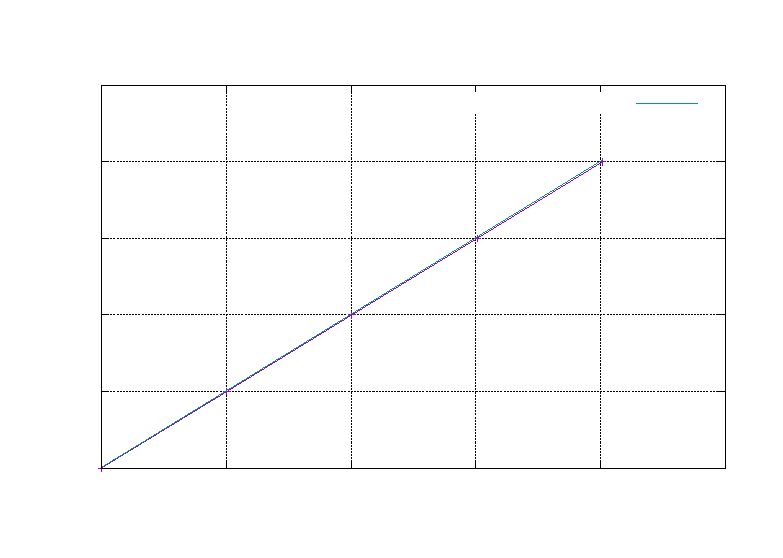
\includegraphics[width={360.00bp},height={252.00bp}]{./Grafy/pierwsza/statyczna/graf}}%
    \gplfronttext
  \end{picture}%
\endgroup

    Te dane pomogą nam wyznaczyć współczynnik sprężystości danej sprężyny. Z prawa Hooke’a wynika, że siła potrzebna do odkształcenia ciała jest wprost proporcjonalna do tego odkształcenia. Można to wyrazić równaniem F = kx, gdzie F jest przykładaną siłą, k jest stałą sprężystości ciała, a x jego wydłużeniem. Pozwala to łatwo wyprowadzić wzór na stałą sprężystości:
    \[k = \frac{F}{x} \]
        Daną x uzyskaliśmy mierząc wydłużenie sprężyny, a F możemy obliczyć za pomocą wzoru na siłę ciężkości F = mg, gdzie m jest masą obciążenia naszej sprężyny, a g jest wartością przyspieszenia grawitacyjnego, która na Ziemi wynosi ok. $9,81 \frac{m}{s^2}$. Po dokonaniu wszystkich obliczeń otrzymaliśmy następujące wyniki:
    
    \pagebreak
    \begin{table}[h!]
        \centering
        \begin{tabular}{|c|c|c|}
            \hline
            Masa ciężarków[kg] & Wydłużenie[m] & stała sprężystości k\\
            \hline
            0.050320 & 0.05 & \pgfmathparse{9.81*0.050320/0.05}\pgfmathresult \\
            \hline
            0.100342 & 0.10 & \pgfmathparse{9.81*0.100342/0.10}\pgfmathresult \\    
            \hline
            0.150596 & 0.15 & \pgfmathparse{9.81*0.150596/0.15}\pgfmathresult \\    
            \hline
            0.200861 & 0.20 & \pgfmathparse{9.81*0.200861/0.20}\pgfmathresult \\  
            \hline
            \multicolumn{2}{|c|}{\textbf{Średnia}} & \pgfmathparse{(9.81*0.050320/0.05 + 9.81*0.100342/0.10 + 9.81*0.150596/0.15 + 9.81*0.200861/0.20) /4}\pgfmathresult \\
            \hline
        \end{tabular}
        \caption{obliczanie stałej k dla poszczególnych pomiarów.}
    \end{table}
    %niepewność pomiaru
    Niepewność pomiaru wydłużenia sprężyny oszacowaliśmy na 0,1 cm.
    Niepewność pomiaru współczynnika sprężystości:
    \\f(x) = 0.081*x + 1.914 \\
    f'(x) = 0.081 \\
    Średnia wartość współczynnika sprężystości sprężyny:
    \[ k = \pgfmathparse{(9.81*0.050320/0.05 + 9.81*0.100342/0.10 + 9.81*0.150596/0.15 + 9.81*0.200861/0.20) /4}\pgfmathresult\]
    Zatem: 
    \[ k = (\pgfmathparse{(9.81*0.050320/0.05 + 9.81*0.100342/0.10 + 9.81*0.150596/0.15 + 9.81*0.200861/0.20) /4}\pgfmathresult \pm  0.081) \frac{N}{m} \]

    \pagebreak
    \textbf{M7.2} Wyznaczyć współczynnik sprężystości wybranej sprężyny wykorzystując
    dynamiczną metodę pomiaru czyli mierząc zależność okresu jej drgań od wartości obciążenia. \\
    % GNUPLOT: LaTeX picture with Postscript
\begingroup
  \makeatletter
  \providecommand\color[2][]{%
    \GenericError{(gnuplot) \space\space\space\@spaces}{%
      Package color not loaded in conjunction with
      terminal option `colourtext'%
    }{See the gnuplot documentation for explanation.%
    }{Either use 'blacktext' in gnuplot or load the package
      color.sty in LaTeX.}%
    \renewcommand\color[2][]{}%
  }%
  \providecommand\includegraphics[2][]{%
    \GenericError{(gnuplot) \space\space\space\@spaces}{%
      Package graphicx or graphics not loaded%
    }{See the gnuplot documentation for explanation.%
    }{The gnuplot epslatex terminal needs graphicx.sty or graphics.sty.}%
    \renewcommand\includegraphics[2][]{}%
  }%
  \providecommand\rotatebox[2]{#2}%
  \@ifundefined{ifGPcolor}{%
    \newif\ifGPcolor
    \GPcolorfalse
  }{}%
  \@ifundefined{ifGPblacktext}{%
    \newif\ifGPblacktext
    \GPblacktexttrue
  }{}%
  % define a \g@addto@macro without @ in the name:
  \let\gplgaddtomacro\g@addto@macro
  % define empty templates for all commands taking text:
  \gdef\gplbacktext{}%
  \gdef\gplfronttext{}%
  \makeatother
  \ifGPblacktext
    % no textcolor at all
    \def\colorrgb#1{}%
    \def\colorgray#1{}%
  \else
    % gray or color?
    \ifGPcolor
      \def\colorrgb#1{\color[rgb]{#1}}%
      \def\colorgray#1{\color[gray]{#1}}%
      \expandafter\def\csname LTw\endcsname{\color{white}}%
      \expandafter\def\csname LTb\endcsname{\color{black}}%
      \expandafter\def\csname LTa\endcsname{\color{black}}%
      \expandafter\def\csname LT0\endcsname{\color[rgb]{1,0,0}}%
      \expandafter\def\csname LT1\endcsname{\color[rgb]{0,1,0}}%
      \expandafter\def\csname LT2\endcsname{\color[rgb]{0,0,1}}%
      \expandafter\def\csname LT3\endcsname{\color[rgb]{1,0,1}}%
      \expandafter\def\csname LT4\endcsname{\color[rgb]{0,1,1}}%
      \expandafter\def\csname LT5\endcsname{\color[rgb]{1,1,0}}%
      \expandafter\def\csname LT6\endcsname{\color[rgb]{0,0,0}}%
      \expandafter\def\csname LT7\endcsname{\color[rgb]{1,0.3,0}}%
      \expandafter\def\csname LT8\endcsname{\color[rgb]{0.5,0.5,0.5}}%
    \else
      % gray
      \def\colorrgb#1{\color{black}}%
      \def\colorgray#1{\color[gray]{#1}}%
      \expandafter\def\csname LTw\endcsname{\color{white}}%
      \expandafter\def\csname LTb\endcsname{\color{black}}%
      \expandafter\def\csname LTa\endcsname{\color{black}}%
      \expandafter\def\csname LT0\endcsname{\color{black}}%
      \expandafter\def\csname LT1\endcsname{\color{black}}%
      \expandafter\def\csname LT2\endcsname{\color{black}}%
      \expandafter\def\csname LT3\endcsname{\color{black}}%
      \expandafter\def\csname LT4\endcsname{\color{black}}%
      \expandafter\def\csname LT5\endcsname{\color{black}}%
      \expandafter\def\csname LT6\endcsname{\color{black}}%
      \expandafter\def\csname LT7\endcsname{\color{black}}%
      \expandafter\def\csname LT8\endcsname{\color{black}}%
    \fi
  \fi
    \setlength{\unitlength}{0.0500bp}%
    \ifx\gptboxheight\undefined%
      \newlength{\gptboxheight}%
      \newlength{\gptboxwidth}%
      \newsavebox{\gptboxtext}%
    \fi%
    \setlength{\fboxrule}{0.5pt}%
    \setlength{\fboxsep}{1pt}%
\begin{picture}(7200.00,5040.00)%
    \gplgaddtomacro\gplbacktext{%
      \csname LTb\endcsname%%
      \put(682,704){\makebox(0,0)[r]{\strut{}$4$}}%
      \csname LTb\endcsname%%
      \put(682,1163){\makebox(0,0)[r]{\strut{}$6$}}%
      \csname LTb\endcsname%%
      \put(682,1623){\makebox(0,0)[r]{\strut{}$8$}}%
      \csname LTb\endcsname%%
      \put(682,2082){\makebox(0,0)[r]{\strut{}$10$}}%
      \csname LTb\endcsname%%
      \put(682,2542){\makebox(0,0)[r]{\strut{}$12$}}%
      \csname LTb\endcsname%%
      \put(682,3001){\makebox(0,0)[r]{\strut{}$14$}}%
      \csname LTb\endcsname%%
      \put(682,3460){\makebox(0,0)[r]{\strut{}$16$}}%
      \csname LTb\endcsname%%
      \put(682,3920){\makebox(0,0)[r]{\strut{}$18$}}%
      \csname LTb\endcsname%%
      \put(682,4379){\makebox(0,0)[r]{\strut{}$20$}}%
      \csname LTb\endcsname%%
      \put(814,484){\makebox(0,0){\strut{}$40$}}%
      \csname LTb\endcsname%%
      \put(1479,484){\makebox(0,0){\strut{}$60$}}%
      \csname LTb\endcsname%%
      \put(2145,484){\makebox(0,0){\strut{}$80$}}%
      \csname LTb\endcsname%%
      \put(2810,484){\makebox(0,0){\strut{}$100$}}%
      \csname LTb\endcsname%%
      \put(3476,484){\makebox(0,0){\strut{}$120$}}%
      \csname LTb\endcsname%%
      \put(4141,484){\makebox(0,0){\strut{}$140$}}%
      \csname LTb\endcsname%%
      \put(4807,484){\makebox(0,0){\strut{}$160$}}%
      \csname LTb\endcsname%%
      \put(5472,484){\makebox(0,0){\strut{}$180$}}%
      \csname LTb\endcsname%%
      \put(6138,484){\makebox(0,0){\strut{}$200$}}%
      \csname LTb\endcsname%%
      \put(6803,484){\makebox(0,0){\strut{}$220$}}%
    }%
    \gplgaddtomacro\gplfronttext{%
      \csname LTb\endcsname%%
      \put(209,2541){\rotatebox{-270}{\makebox(0,0){\strut{}Czas wykonywania 20 wachań[s]}}}%
      \put(3808,154){\makebox(0,0){\strut{}Masa ciężarków[g]}}%
      \csname LTb\endcsname%%
      \put(5816,4206){\makebox(0,0)[r]{\strut{}$0.081*x + 1.914$}}%
      \csname LTb\endcsname%%
      \put(3808,4709){\makebox(0,0){\strut{}Otrzymane wyniki za pomocą metody dynamicznej}}%
    }%
    \gplbacktext
    \put(0,0){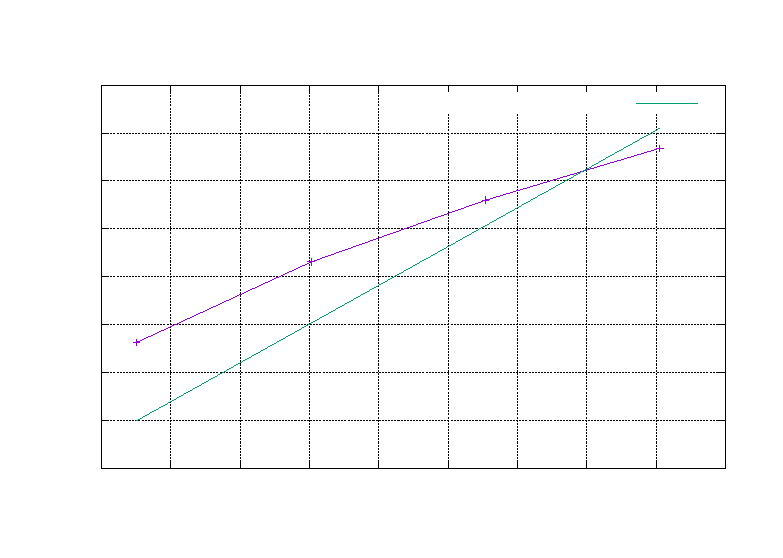
\includegraphics[width={360.00bp},height={252.00bp}]{./Grafy/pierwsza/dynamiczna/graf}}%
    \gplfronttext
  \end{picture}%
\endgroup

    
    używając \[ k = \frac{4 \pi ^2 m}{T^2} \]
    
    \begin{table}[h!]
        \centering
        \begin{tabular}{|c|c|c|c|}
            \hline
            Masa ciężarków[kg] & \rrtabname & \Ts & stała sprężystości k\\
            \hline
            0.050152 & 9.25 & \pgfmath{(9.31+9.21+9.23)/3/20} & \pgfmathparse{4*(3.14)^2 * 0.050152  / ((9.31+9.21+9.23)/(3*20))^2}\pgfmathresult\\  
            \hline
            0.100508 & 12.61 & \pgfmath{(12.59+12.68+12.56)/3/20} & \pgfmathparse{4*(3.14)^2 * 0.100508  / ((12.59+12.68+12.56)/(3*20))^2}\pgfmathresult\\    
            \hline
            0.150830 & 15.19 & \pgfmath{(15.25+15.17+15.16)/3/20} & \pgfmathparse{4*(3.14)^2 * 0.150830  / ((15.25+15.17+15.16)/(3*20))^2}\pgfmathresult\\    
            \hline
            0.201095 & 17.36 & \pgfmath{(17.40+17.41+17.28)/3/20} & \pgfmathparse{4*(3.14)^2 * 0.201095  / ((17.40+17.41+17.28)/(3*20))^2}\pgfmathresult\\  
            \hline
            \multicolumn{3}{|c|}{\textbf{Średnia}} & \pgfmathparse{((4*(3.14)^2 * 0.050152  / ((9.31+9.21+9.23)/(3*20))^2) + (4*(3.14)^2 * 0.100508  / ((12.59+12.68+12.56)/(3*20))^2) + (4*(3.14)^2 * 0.150830  / ((15.25+15.17+15.16)/(3*20))^2) + (4*(3.14)^2 * 0.201095  / ((17.40+17.41+17.28)/(3*20))^2))/4}\pgfmathresult \\
            \hline
        \end{tabular}
    \end{table}
    %niepewność pomiaru
    Niepewność pomiaru wydłużenia sprężyny oszacowaliśmy na 0,1 cm.
    Niepewność pomiaru współczynnika sprężystości:
    \\f(x) = 0.081*x + 1.914 \\
    f'(x) = 0.081 \\
    Średnia wartość współczynnika sprężystości sprężyny:
    \[ k = \pgfmathparse{((4*(3.14)^2 * 0.050152  / ((9.31+9.21+9.23)/(3*20))^2) + (4*(3.14)^2 * 0.100508  / ((12.59+12.68+12.56)/(3*20))^2) + (4*(3.14)^2 * 0.150830  / ((15.25+15.17+15.16)/(3*20))^2) + (4*(3.14)^2 * 0.201095  / ((17.40+17.41+17.28)/(3*20))^2))/4}\pgfmathresult \]
    Zatem: 
    \[ k = (\pgfmathparse{((4*(3.14)^2 * 0.050152  / ((9.31+9.21+9.23)/(3*20))^2) + (4*(3.14)^2 * 0.100508  / ((12.59+12.68+12.56)/(3*20))^2) + (4*(3.14)^2 * 0.150830  / ((15.25+15.17+15.16)/(3*20))^2) + (4*(3.14)^2 * 0.201095  / ((17.40+17.41+17.28)/(3*20))^2))/4}\pgfmathresult \pm  0.081) \frac{N}{m} \]
    
    
    \textbf{M7.3} Obliczyć moduł sztywności materiału sprężyny.\\
    Współczynnik sprężystości sprężyny jest zależny od modułu sztywności materiału, z którego została zrobiona, na co wskazuje równanie $k = \frac{Gr^4}{4NR^3}$. W celu obliczenia modułu, można go wyprowadzić z tego wzoru by uzyskać takie równanie: 
    \[G = \frac{4kNR^3}{r^4}\]
    gdzie:\\
    k - współczynnik sprężystości sprężyny,\\
    N - liczba zwojów sprężyny,\\
    R - promień sprężyny,\\
    r - promień drutu sprężyny.\\
    \[ G = \frac{ \pgfmathparse{(9.81*0.050320/0.05 + 9.81*0.100342/0.10 + 9.81*0.150596/0.15 + 9.81*0.200861/0.20) /4}\pgfmathresult*4 * 77 * 0.0083^3}{0.0004^4} = 67.7918 GPa\]
    
    \pagebreak
    \textbf{Obliczenia dla zadań M7.4. - M7.5.} \\
    
    Obliczamy współczynnik sprężystości dla drugiej sprężyny, aby porównać czy teoretyczny współczynnik sprężystości układu sprężyn jest zgodny z pomiarem.
    
    % GNUPLOT: LaTeX picture with Postscript
\begingroup
  \makeatletter
  \providecommand\color[2][]{%
    \GenericError{(gnuplot) \space\space\space\@spaces}{%
      Package color not loaded in conjunction with
      terminal option `colourtext'%
    }{See the gnuplot documentation for explanation.%
    }{Either use 'blacktext' in gnuplot or load the package
      color.sty in LaTeX.}%
    \renewcommand\color[2][]{}%
  }%
  \providecommand\includegraphics[2][]{%
    \GenericError{(gnuplot) \space\space\space\@spaces}{%
      Package graphicx or graphics not loaded%
    }{See the gnuplot documentation for explanation.%
    }{The gnuplot epslatex terminal needs graphicx.sty or graphics.sty.}%
    \renewcommand\includegraphics[2][]{}%
  }%
  \providecommand\rotatebox[2]{#2}%
  \@ifundefined{ifGPcolor}{%
    \newif\ifGPcolor
    \GPcolorfalse
  }{}%
  \@ifundefined{ifGPblacktext}{%
    \newif\ifGPblacktext
    \GPblacktexttrue
  }{}%
  % define a \g@addto@macro without @ in the name:
  \let\gplgaddtomacro\g@addto@macro
  % define empty templates for all commands taking text:
  \gdef\gplbacktext{}%
  \gdef\gplfronttext{}%
  \makeatother
  \ifGPblacktext
    % no textcolor at all
    \def\colorrgb#1{}%
    \def\colorgray#1{}%
  \else
    % gray or color?
    \ifGPcolor
      \def\colorrgb#1{\color[rgb]{#1}}%
      \def\colorgray#1{\color[gray]{#1}}%
      \expandafter\def\csname LTw\endcsname{\color{white}}%
      \expandafter\def\csname LTb\endcsname{\color{black}}%
      \expandafter\def\csname LTa\endcsname{\color{black}}%
      \expandafter\def\csname LT0\endcsname{\color[rgb]{1,0,0}}%
      \expandafter\def\csname LT1\endcsname{\color[rgb]{0,1,0}}%
      \expandafter\def\csname LT2\endcsname{\color[rgb]{0,0,1}}%
      \expandafter\def\csname LT3\endcsname{\color[rgb]{1,0,1}}%
      \expandafter\def\csname LT4\endcsname{\color[rgb]{0,1,1}}%
      \expandafter\def\csname LT5\endcsname{\color[rgb]{1,1,0}}%
      \expandafter\def\csname LT6\endcsname{\color[rgb]{0,0,0}}%
      \expandafter\def\csname LT7\endcsname{\color[rgb]{1,0.3,0}}%
      \expandafter\def\csname LT8\endcsname{\color[rgb]{0.5,0.5,0.5}}%
    \else
      % gray
      \def\colorrgb#1{\color{black}}%
      \def\colorgray#1{\color[gray]{#1}}%
      \expandafter\def\csname LTw\endcsname{\color{white}}%
      \expandafter\def\csname LTb\endcsname{\color{black}}%
      \expandafter\def\csname LTa\endcsname{\color{black}}%
      \expandafter\def\csname LT0\endcsname{\color{black}}%
      \expandafter\def\csname LT1\endcsname{\color{black}}%
      \expandafter\def\csname LT2\endcsname{\color{black}}%
      \expandafter\def\csname LT3\endcsname{\color{black}}%
      \expandafter\def\csname LT4\endcsname{\color{black}}%
      \expandafter\def\csname LT5\endcsname{\color{black}}%
      \expandafter\def\csname LT6\endcsname{\color{black}}%
      \expandafter\def\csname LT7\endcsname{\color{black}}%
      \expandafter\def\csname LT8\endcsname{\color{black}}%
    \fi
  \fi
    \setlength{\unitlength}{0.0500bp}%
    \ifx\gptboxheight\undefined%
      \newlength{\gptboxheight}%
      \newlength{\gptboxwidth}%
      \newsavebox{\gptboxtext}%
    \fi%
    \setlength{\fboxrule}{0.5pt}%
    \setlength{\fboxsep}{1pt}%
\begin{picture}(7200.00,5040.00)%
    \gplgaddtomacro\gplbacktext{%
      \csname LTb\endcsname%%
      \put(682,704){\makebox(0,0)[r]{\strut{}$-5$}}%
      \csname LTb\endcsname%%
      \put(682,1317){\makebox(0,0)[r]{\strut{}$0$}}%
      \csname LTb\endcsname%%
      \put(682,1929){\makebox(0,0)[r]{\strut{}$5$}}%
      \csname LTb\endcsname%%
      \put(682,2542){\makebox(0,0)[r]{\strut{}$10$}}%
      \csname LTb\endcsname%%
      \put(682,3154){\makebox(0,0)[r]{\strut{}$15$}}%
      \csname LTb\endcsname%%
      \put(682,3767){\makebox(0,0)[r]{\strut{}$20$}}%
      \csname LTb\endcsname%%
      \put(682,4379){\makebox(0,0)[r]{\strut{}$25$}}%
      \csname LTb\endcsname%%
      \put(814,484){\makebox(0,0){\strut{}$0$}}%
      \csname LTb\endcsname%%
      \put(2012,484){\makebox(0,0){\strut{}$50$}}%
      \csname LTb\endcsname%%
      \put(3210,484){\makebox(0,0){\strut{}$100$}}%
      \csname LTb\endcsname%%
      \put(4407,484){\makebox(0,0){\strut{}$150$}}%
      \csname LTb\endcsname%%
      \put(5605,484){\makebox(0,0){\strut{}$200$}}%
      \csname LTb\endcsname%%
      \put(6803,484){\makebox(0,0){\strut{}$250$}}%
    }%
    \gplgaddtomacro\gplfronttext{%
      \csname LTb\endcsname%%
      \put(209,2541){\rotatebox{-270}{\makebox(0,0){\strut{}Wydłużenie[cm]}}}%
      \put(3808,154){\makebox(0,0){\strut{}Masa ciężarków[g]}}%
      \csname LTb\endcsname%%
      \put(5816,4206){\makebox(0,0)[r]{\strut{}$0.103*x + -0.258$}}%
      \csname LTb\endcsname%%
      \put(3808,4709){\makebox(0,0){\strut{}Otrzymane wyniki za pomocą metody statycznej}}%
    }%
    \gplbacktext
    \put(0,0){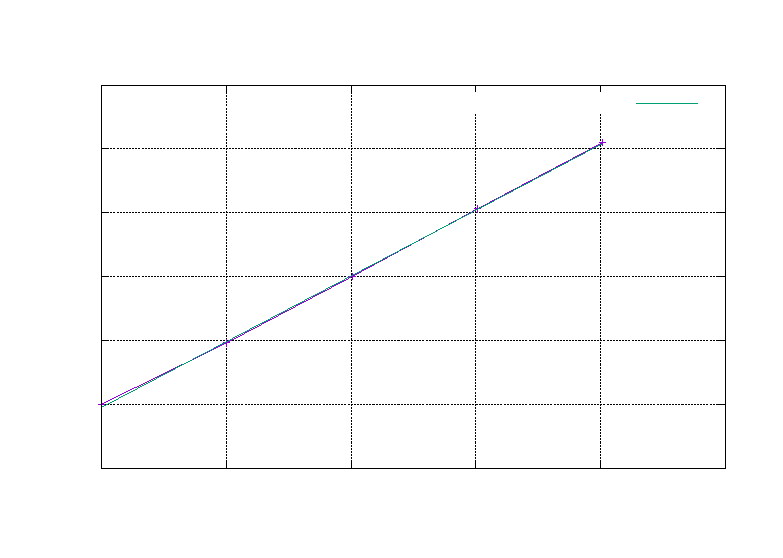
\includegraphics[width={360.00bp},height={252.00bp}]{./Grafy/druga/statyczna/graf}}%
    \gplfronttext
  \end{picture}%
\endgroup

    \begin{table}[h!]
        \centering
        \begin{tabular}{|c|c|c|}
            \hline
            Masa ciężarków[kg] & Wydłużenie[m] & Stała sprężystości k\\
            \hline
            0.050155  & 0.048 & \pgfmathparse{9.81*0.050155/0.048}\pgfmathresult\\  
            \hline
            0.100478  & 0.100 & \pgfmathparse{9.81*0.100478/0.100}\pgfmathresult\\    
            \hline
            0.150614 & 0.153 & \pgfmathparse{9.81*0.150614/0.153}\pgfmathresult\\    
            \hline
            0.200790 & 0.205 & \pgfmathparse{9.81*0.200790/0.205}\pgfmathresult\\  
            \hline
            \multicolumn{2}{|c|}{\textbf{Średnia}} & \pgfmathparse{(9.81*0.050155/0.048 + 9.81*0.100478/0.100 + 9.81*0.150614/0.153 + 9.81*0.200790/0.205)/4}\pgfmathresult \\
            \hline
        \end{tabular}
        \caption{obliczanie stałej k dla poszczególnych pomiarów.}
    \end{table}

    % GNUPLOT: LaTeX picture with Postscript
\begingroup
  \makeatletter
  \providecommand\color[2][]{%
    \GenericError{(gnuplot) \space\space\space\@spaces}{%
      Package color not loaded in conjunction with
      terminal option `colourtext'%
    }{See the gnuplot documentation for explanation.%
    }{Either use 'blacktext' in gnuplot or load the package
      color.sty in LaTeX.}%
    \renewcommand\color[2][]{}%
  }%
  \providecommand\includegraphics[2][]{%
    \GenericError{(gnuplot) \space\space\space\@spaces}{%
      Package graphicx or graphics not loaded%
    }{See the gnuplot documentation for explanation.%
    }{The gnuplot epslatex terminal needs graphicx.sty or graphics.sty.}%
    \renewcommand\includegraphics[2][]{}%
  }%
  \providecommand\rotatebox[2]{#2}%
  \@ifundefined{ifGPcolor}{%
    \newif\ifGPcolor
    \GPcolorfalse
  }{}%
  \@ifundefined{ifGPblacktext}{%
    \newif\ifGPblacktext
    \GPblacktexttrue
  }{}%
  % define a \g@addto@macro without @ in the name:
  \let\gplgaddtomacro\g@addto@macro
  % define empty templates for all commands taking text:
  \gdef\gplbacktext{}%
  \gdef\gplfronttext{}%
  \makeatother
  \ifGPblacktext
    % no textcolor at all
    \def\colorrgb#1{}%
    \def\colorgray#1{}%
  \else
    % gray or color?
    \ifGPcolor
      \def\colorrgb#1{\color[rgb]{#1}}%
      \def\colorgray#1{\color[gray]{#1}}%
      \expandafter\def\csname LTw\endcsname{\color{white}}%
      \expandafter\def\csname LTb\endcsname{\color{black}}%
      \expandafter\def\csname LTa\endcsname{\color{black}}%
      \expandafter\def\csname LT0\endcsname{\color[rgb]{1,0,0}}%
      \expandafter\def\csname LT1\endcsname{\color[rgb]{0,1,0}}%
      \expandafter\def\csname LT2\endcsname{\color[rgb]{0,0,1}}%
      \expandafter\def\csname LT3\endcsname{\color[rgb]{1,0,1}}%
      \expandafter\def\csname LT4\endcsname{\color[rgb]{0,1,1}}%
      \expandafter\def\csname LT5\endcsname{\color[rgb]{1,1,0}}%
      \expandafter\def\csname LT6\endcsname{\color[rgb]{0,0,0}}%
      \expandafter\def\csname LT7\endcsname{\color[rgb]{1,0.3,0}}%
      \expandafter\def\csname LT8\endcsname{\color[rgb]{0.5,0.5,0.5}}%
    \else
      % gray
      \def\colorrgb#1{\color{black}}%
      \def\colorgray#1{\color[gray]{#1}}%
      \expandafter\def\csname LTw\endcsname{\color{white}}%
      \expandafter\def\csname LTb\endcsname{\color{black}}%
      \expandafter\def\csname LTa\endcsname{\color{black}}%
      \expandafter\def\csname LT0\endcsname{\color{black}}%
      \expandafter\def\csname LT1\endcsname{\color{black}}%
      \expandafter\def\csname LT2\endcsname{\color{black}}%
      \expandafter\def\csname LT3\endcsname{\color{black}}%
      \expandafter\def\csname LT4\endcsname{\color{black}}%
      \expandafter\def\csname LT5\endcsname{\color{black}}%
      \expandafter\def\csname LT6\endcsname{\color{black}}%
      \expandafter\def\csname LT7\endcsname{\color{black}}%
      \expandafter\def\csname LT8\endcsname{\color{black}}%
    \fi
  \fi
    \setlength{\unitlength}{0.0500bp}%
    \ifx\gptboxheight\undefined%
      \newlength{\gptboxheight}%
      \newlength{\gptboxwidth}%
      \newsavebox{\gptboxtext}%
    \fi%
    \setlength{\fboxrule}{0.5pt}%
    \setlength{\fboxsep}{1pt}%
\begin{picture}(7200.00,5040.00)%
    \gplgaddtomacro\gplbacktext{%
      \csname LTb\endcsname%%
      \put(682,704){\makebox(0,0)[r]{\strut{}$9$}}%
      \csname LTb\endcsname%%
      \put(682,1112){\makebox(0,0)[r]{\strut{}$10$}}%
      \csname LTb\endcsname%%
      \put(682,1521){\makebox(0,0)[r]{\strut{}$11$}}%
      \csname LTb\endcsname%%
      \put(682,1929){\makebox(0,0)[r]{\strut{}$12$}}%
      \csname LTb\endcsname%%
      \put(682,2337){\makebox(0,0)[r]{\strut{}$13$}}%
      \csname LTb\endcsname%%
      \put(682,2746){\makebox(0,0)[r]{\strut{}$14$}}%
      \csname LTb\endcsname%%
      \put(682,3154){\makebox(0,0)[r]{\strut{}$15$}}%
      \csname LTb\endcsname%%
      \put(682,3562){\makebox(0,0)[r]{\strut{}$16$}}%
      \csname LTb\endcsname%%
      \put(682,3971){\makebox(0,0)[r]{\strut{}$17$}}%
      \csname LTb\endcsname%%
      \put(682,4379){\makebox(0,0)[r]{\strut{}$18$}}%
      \csname LTb\endcsname%%
      \put(814,484){\makebox(0,0){\strut{}$40$}}%
      \csname LTb\endcsname%%
      \put(1479,484){\makebox(0,0){\strut{}$60$}}%
      \csname LTb\endcsname%%
      \put(2145,484){\makebox(0,0){\strut{}$80$}}%
      \csname LTb\endcsname%%
      \put(2810,484){\makebox(0,0){\strut{}$100$}}%
      \csname LTb\endcsname%%
      \put(3476,484){\makebox(0,0){\strut{}$120$}}%
      \csname LTb\endcsname%%
      \put(4141,484){\makebox(0,0){\strut{}$140$}}%
      \csname LTb\endcsname%%
      \put(4807,484){\makebox(0,0){\strut{}$160$}}%
      \csname LTb\endcsname%%
      \put(5472,484){\makebox(0,0){\strut{}$180$}}%
      \csname LTb\endcsname%%
      \put(6138,484){\makebox(0,0){\strut{}$200$}}%
      \csname LTb\endcsname%%
      \put(6803,484){\makebox(0,0){\strut{}$220$}}%
    }%
    \gplgaddtomacro\gplfronttext{%
      \csname LTb\endcsname%%
      \put(209,2541){\rotatebox{-270}{\makebox(0,0){\strut{}Czas wykonywania 20 wachań[s]}}}%
      \put(3808,154){\makebox(0,0){\strut{}Masa ciężarków[cm]}}%
      \csname LTb\endcsname%%
      \put(3808,4709){\makebox(0,0){\strut{}Otrzymane wyniki za pomocą metody dynamicznej}}%
    }%
    \gplbacktext
    \put(0,0){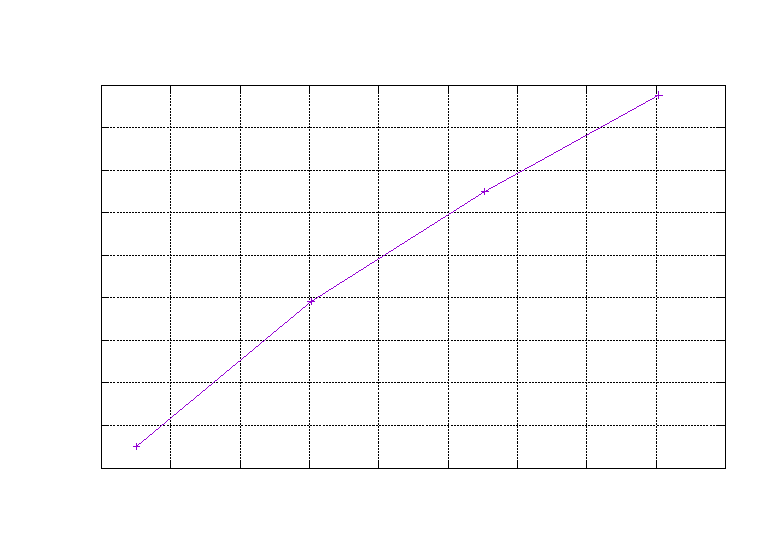
\includegraphics[width={360.00bp},height={252.00bp}]{./Grafy/druga/dynamiczna/graf}}%
    \gplfronttext
  \end{picture}%
\endgroup

    \begin{table}[h!]
        \centering
        \begin{tabular}{|c|c|c|c|}
            \hline
            Masa ciężarków[kg] & \rrtabname & \Ts & Stała sprężystości k\\
            \hline
            0.050155 & 9.51 & \pgfmath{(9.53+9.49)/2/20} & \pgfmathparse{4*(3.14)^2 * 0.050155  / ((9.53+9.49)/(2*20))^2}\pgfmathresult\\  
            \hline
            0.100478 & 12.91 & \pgfmath{(12.89+12.93)/2/20} & \pgfmathparse{4*(3.14)^2 * 0.100478  / ((12.89+12.93)/(2*20))^2}\pgfmathresult\\    
            \hline
            0.150614 & 15.50 & \pgfmath{(15.57+15.43)/2/20} & \pgfmathparse{4*(3.14)^2 * 0.150614  / ((15.57+15.43)/(2*20))^2}\pgfmathresult\\    
            \hline
            0.200790 & 17.77 & \pgfmath{(17.76+17.77)/2/20} & \pgfmathparse{4*(3.14)^2 * 0.200790  / ((17.76+17.77)/(2*20))^2}\pgfmathresult\\  
            \hline
            \multicolumn{3}{|c|}{\textbf{Średnia}} & \pgfmathparse{((4*(3.14)^2 * 0.050155  / ((9.53+9.49)/(2*20))^2) + (4*(3.14)^2 * 0.100478  / ((12.89+12.93)/(2*20))^2) + (4*(3.14)^2 * 0.150614  / ((15.57+15.43)/(2*20))^2) + (4*(3.14)^2 * 0.200790  / ((17.76+17.77)/(2*20))^2))/4}\pgfmathresult \\
            \hline
        \end{tabular}
    \end{table}

    \pagebreak
    \textbf{M7.4}
    Wyznaczanie współczynnika sprężystości sprężyn połączonych równolegle \\
    
    \textbf{a)}
    Metoda statyczna \\
    % GNUPLOT: LaTeX picture with Postscript
\begingroup
  \makeatletter
  \providecommand\color[2][]{%
    \GenericError{(gnuplot) \space\space\space\@spaces}{%
      Package color not loaded in conjunction with
      terminal option `colourtext'%
    }{See the gnuplot documentation for explanation.%
    }{Either use 'blacktext' in gnuplot or load the package
      color.sty in LaTeX.}%
    \renewcommand\color[2][]{}%
  }%
  \providecommand\includegraphics[2][]{%
    \GenericError{(gnuplot) \space\space\space\@spaces}{%
      Package graphicx or graphics not loaded%
    }{See the gnuplot documentation for explanation.%
    }{The gnuplot epslatex terminal needs graphicx.sty or graphics.sty.}%
    \renewcommand\includegraphics[2][]{}%
  }%
  \providecommand\rotatebox[2]{#2}%
  \@ifundefined{ifGPcolor}{%
    \newif\ifGPcolor
    \GPcolorfalse
  }{}%
  \@ifundefined{ifGPblacktext}{%
    \newif\ifGPblacktext
    \GPblacktexttrue
  }{}%
  % define a \g@addto@macro without @ in the name:
  \let\gplgaddtomacro\g@addto@macro
  % define empty templates for all commands taking text:
  \gdef\gplbacktext{}%
  \gdef\gplfronttext{}%
  \makeatother
  \ifGPblacktext
    % no textcolor at all
    \def\colorrgb#1{}%
    \def\colorgray#1{}%
  \else
    % gray or color?
    \ifGPcolor
      \def\colorrgb#1{\color[rgb]{#1}}%
      \def\colorgray#1{\color[gray]{#1}}%
      \expandafter\def\csname LTw\endcsname{\color{white}}%
      \expandafter\def\csname LTb\endcsname{\color{black}}%
      \expandafter\def\csname LTa\endcsname{\color{black}}%
      \expandafter\def\csname LT0\endcsname{\color[rgb]{1,0,0}}%
      \expandafter\def\csname LT1\endcsname{\color[rgb]{0,1,0}}%
      \expandafter\def\csname LT2\endcsname{\color[rgb]{0,0,1}}%
      \expandafter\def\csname LT3\endcsname{\color[rgb]{1,0,1}}%
      \expandafter\def\csname LT4\endcsname{\color[rgb]{0,1,1}}%
      \expandafter\def\csname LT5\endcsname{\color[rgb]{1,1,0}}%
      \expandafter\def\csname LT6\endcsname{\color[rgb]{0,0,0}}%
      \expandafter\def\csname LT7\endcsname{\color[rgb]{1,0.3,0}}%
      \expandafter\def\csname LT8\endcsname{\color[rgb]{0.5,0.5,0.5}}%
    \else
      % gray
      \def\colorrgb#1{\color{black}}%
      \def\colorgray#1{\color[gray]{#1}}%
      \expandafter\def\csname LTw\endcsname{\color{white}}%
      \expandafter\def\csname LTb\endcsname{\color{black}}%
      \expandafter\def\csname LTa\endcsname{\color{black}}%
      \expandafter\def\csname LT0\endcsname{\color{black}}%
      \expandafter\def\csname LT1\endcsname{\color{black}}%
      \expandafter\def\csname LT2\endcsname{\color{black}}%
      \expandafter\def\csname LT3\endcsname{\color{black}}%
      \expandafter\def\csname LT4\endcsname{\color{black}}%
      \expandafter\def\csname LT5\endcsname{\color{black}}%
      \expandafter\def\csname LT6\endcsname{\color{black}}%
      \expandafter\def\csname LT7\endcsname{\color{black}}%
      \expandafter\def\csname LT8\endcsname{\color{black}}%
    \fi
  \fi
    \setlength{\unitlength}{0.0500bp}%
    \ifx\gptboxheight\undefined%
      \newlength{\gptboxheight}%
      \newlength{\gptboxwidth}%
      \newsavebox{\gptboxtext}%
    \fi%
    \setlength{\fboxrule}{0.5pt}%
    \setlength{\fboxsep}{1pt}%
\begin{picture}(7200.00,5040.00)%
    \gplgaddtomacro\gplbacktext{%
      \csname LTb\endcsname%%
      \put(682,704){\makebox(0,0)[r]{\strut{}$-2$}}%
      \csname LTb\endcsname%%
      \put(682,1229){\makebox(0,0)[r]{\strut{}$0$}}%
      \csname LTb\endcsname%%
      \put(682,1754){\makebox(0,0)[r]{\strut{}$2$}}%
      \csname LTb\endcsname%%
      \put(682,2279){\makebox(0,0)[r]{\strut{}$4$}}%
      \csname LTb\endcsname%%
      \put(682,2804){\makebox(0,0)[r]{\strut{}$6$}}%
      \csname LTb\endcsname%%
      \put(682,3329){\makebox(0,0)[r]{\strut{}$8$}}%
      \csname LTb\endcsname%%
      \put(682,3854){\makebox(0,0)[r]{\strut{}$10$}}%
      \csname LTb\endcsname%%
      \put(682,4379){\makebox(0,0)[r]{\strut{}$12$}}%
      \csname LTb\endcsname%%
      \put(814,484){\makebox(0,0){\strut{}$0$}}%
      \csname LTb\endcsname%%
      \put(2012,484){\makebox(0,0){\strut{}$50$}}%
      \csname LTb\endcsname%%
      \put(3210,484){\makebox(0,0){\strut{}$100$}}%
      \csname LTb\endcsname%%
      \put(4407,484){\makebox(0,0){\strut{}$150$}}%
      \csname LTb\endcsname%%
      \put(5605,484){\makebox(0,0){\strut{}$200$}}%
      \csname LTb\endcsname%%
      \put(6803,484){\makebox(0,0){\strut{}$250$}}%
    }%
    \gplgaddtomacro\gplfronttext{%
      \csname LTb\endcsname%%
      \put(209,2541){\rotatebox{-270}{\makebox(0,0){\strut{}Wydłużenie[cm]}}}%
      \put(3808,154){\makebox(0,0){\strut{}Masa ciężarków[g]}}%
      \csname LTb\endcsname%%
      \put(5816,4206){\makebox(0,0)[r]{\strut{}$0.051*x + -0.119$}}%
      \csname LTb\endcsname%%
      \put(3808,4709){\makebox(0,0){\strut{}Otrzymane wyniki za pomocą metody statycznej}}%
    }%
    \gplbacktext
    \put(0,0){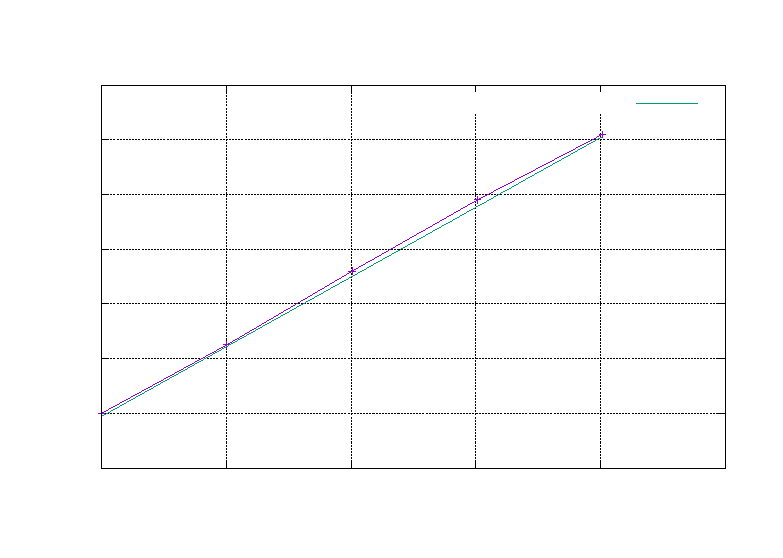
\includegraphics[width={360.00bp},height={252.00bp}]{./Grafy/szeregowo/statyczna/graf}}%
    \gplfronttext
  \end{picture}%
\endgroup

    \begin{table}[h!]
        \centering
        \begin{tabular}{|c|c|c|}
            \hline
            Masa ciężarków[kg] & Wydłużenie[m] & stała sprężystości k\\
            \hline
            0.050155  & 0.025 & \pgfmathparse{9.81*0.050155/0.025}\pgfmathresult\\  
            \hline
            0.100478  & 0.052 & \pgfmathparse{9.81*0.100478/0.052}\pgfmathresult\\    
            \hline
            0.150614 & 0.078 & \pgfmathparse{9.81*0.150614/0.078}\pgfmathresult\\    
            \hline
            0.200790 & 0.102 & \pgfmathparse{9.81*0.200790/0.102}\pgfmathresult\\  
            \hline
            \multicolumn{2}{|c|}{\textbf{Średnia}} & \pgfmathparse{(9.81*0.050155/0.025 + 9.81*0.100478/0.052 + 9.81*0.150614/0.078 + 9.81*0.200790/0.102)/4}\pgfmathresult \\
            \hline
        \end{tabular}
        \caption{obliczanie stałej k dla poszczególnych pomiarów.}
    \end{table}
    
    %niepewność pomiaru
    Niepewność pomiaru wydłużenia sprężyny oszacowaliśmy na 0,1 cm.
    Niepewność pomiaru współczynnika sprężystości:
    \\f(x) = 0.051*x - 0.119 \\
    f'(x) = 0.051 \\
    Średnia wartość współczynnika sprężystości sprężyny:
    \[ k = \pgfmathparse{(9.81*0.050155/0.025 + 9.81*0.100478/0.052 + 9.81*0.150614/0.078 + 9.81*0.200790/0.102)/4}\pgfmathresult\ \]
    Zatem: 
    \[ k = (\pgfmathparse{(9.81*0.050155/0.025 + 9.81*0.100478/0.052 + 9.81*0.150614/0.078 + 9.81*0.200790/0.102)/4}\pgfmathresult\ \pm  0.081) \frac{N}{m} \]
    
    Korzystając ze wzoru $k = k_1 + k_2$ możemy obliczyć teoretyczną wartość współczynnika sprężystości w celu porównania i sprawdzenia czy nasze pomiary są prawidłowe.
    \[ k = 9.85445 +  9.84338 = \pgfmathparse{9.85445 +  9.84338}\pgfmathresult\]
    Wynik mierzony bliski jest temu teoretycznemu. \\

    \textbf{b)}
    Metoda dynamiczna \\
    % GNUPLOT: LaTeX picture with Postscript
\begingroup
  \makeatletter
  \providecommand\color[2][]{%
    \GenericError{(gnuplot) \space\space\space\@spaces}{%
      Package color not loaded in conjunction with
      terminal option `colourtext'%
    }{See the gnuplot documentation for explanation.%
    }{Either use 'blacktext' in gnuplot or load the package
      color.sty in LaTeX.}%
    \renewcommand\color[2][]{}%
  }%
  \providecommand\includegraphics[2][]{%
    \GenericError{(gnuplot) \space\space\space\@spaces}{%
      Package graphicx or graphics not loaded%
    }{See the gnuplot documentation for explanation.%
    }{The gnuplot epslatex terminal needs graphicx.sty or graphics.sty.}%
    \renewcommand\includegraphics[2][]{}%
  }%
  \providecommand\rotatebox[2]{#2}%
  \@ifundefined{ifGPcolor}{%
    \newif\ifGPcolor
    \GPcolorfalse
  }{}%
  \@ifundefined{ifGPblacktext}{%
    \newif\ifGPblacktext
    \GPblacktexttrue
  }{}%
  % define a \g@addto@macro without @ in the name:
  \let\gplgaddtomacro\g@addto@macro
  % define empty templates for all commands taking text:
  \gdef\gplbacktext{}%
  \gdef\gplfronttext{}%
  \makeatother
  \ifGPblacktext
    % no textcolor at all
    \def\colorrgb#1{}%
    \def\colorgray#1{}%
  \else
    % gray or color?
    \ifGPcolor
      \def\colorrgb#1{\color[rgb]{#1}}%
      \def\colorgray#1{\color[gray]{#1}}%
      \expandafter\def\csname LTw\endcsname{\color{white}}%
      \expandafter\def\csname LTb\endcsname{\color{black}}%
      \expandafter\def\csname LTa\endcsname{\color{black}}%
      \expandafter\def\csname LT0\endcsname{\color[rgb]{1,0,0}}%
      \expandafter\def\csname LT1\endcsname{\color[rgb]{0,1,0}}%
      \expandafter\def\csname LT2\endcsname{\color[rgb]{0,0,1}}%
      \expandafter\def\csname LT3\endcsname{\color[rgb]{1,0,1}}%
      \expandafter\def\csname LT4\endcsname{\color[rgb]{0,1,1}}%
      \expandafter\def\csname LT5\endcsname{\color[rgb]{1,1,0}}%
      \expandafter\def\csname LT6\endcsname{\color[rgb]{0,0,0}}%
      \expandafter\def\csname LT7\endcsname{\color[rgb]{1,0.3,0}}%
      \expandafter\def\csname LT8\endcsname{\color[rgb]{0.5,0.5,0.5}}%
    \else
      % gray
      \def\colorrgb#1{\color{black}}%
      \def\colorgray#1{\color[gray]{#1}}%
      \expandafter\def\csname LTw\endcsname{\color{white}}%
      \expandafter\def\csname LTb\endcsname{\color{black}}%
      \expandafter\def\csname LTa\endcsname{\color{black}}%
      \expandafter\def\csname LT0\endcsname{\color{black}}%
      \expandafter\def\csname LT1\endcsname{\color{black}}%
      \expandafter\def\csname LT2\endcsname{\color{black}}%
      \expandafter\def\csname LT3\endcsname{\color{black}}%
      \expandafter\def\csname LT4\endcsname{\color{black}}%
      \expandafter\def\csname LT5\endcsname{\color{black}}%
      \expandafter\def\csname LT6\endcsname{\color{black}}%
      \expandafter\def\csname LT7\endcsname{\color{black}}%
      \expandafter\def\csname LT8\endcsname{\color{black}}%
    \fi
  \fi
    \setlength{\unitlength}{0.0500bp}%
    \ifx\gptboxheight\undefined%
      \newlength{\gptboxheight}%
      \newlength{\gptboxwidth}%
      \newsavebox{\gptboxtext}%
    \fi%
    \setlength{\fboxrule}{0.5pt}%
    \setlength{\fboxsep}{1pt}%
\begin{picture}(7200.00,5040.00)%
    \gplgaddtomacro\gplbacktext{%
      \csname LTb\endcsname%%
      \put(682,704){\makebox(0,0)[r]{\strut{}$4$}}%
      \csname LTb\endcsname%%
      \put(682,1038){\makebox(0,0)[r]{\strut{}$5$}}%
      \csname LTb\endcsname%%
      \put(682,1372){\makebox(0,0)[r]{\strut{}$6$}}%
      \csname LTb\endcsname%%
      \put(682,1706){\makebox(0,0)[r]{\strut{}$7$}}%
      \csname LTb\endcsname%%
      \put(682,2040){\makebox(0,0)[r]{\strut{}$8$}}%
      \csname LTb\endcsname%%
      \put(682,2374){\makebox(0,0)[r]{\strut{}$9$}}%
      \csname LTb\endcsname%%
      \put(682,2709){\makebox(0,0)[r]{\strut{}$10$}}%
      \csname LTb\endcsname%%
      \put(682,3043){\makebox(0,0)[r]{\strut{}$11$}}%
      \csname LTb\endcsname%%
      \put(682,3377){\makebox(0,0)[r]{\strut{}$12$}}%
      \csname LTb\endcsname%%
      \put(682,3711){\makebox(0,0)[r]{\strut{}$13$}}%
      \csname LTb\endcsname%%
      \put(682,4045){\makebox(0,0)[r]{\strut{}$14$}}%
      \csname LTb\endcsname%%
      \put(682,4379){\makebox(0,0)[r]{\strut{}$15$}}%
      \csname LTb\endcsname%%
      \put(814,484){\makebox(0,0){\strut{}$40$}}%
      \csname LTb\endcsname%%
      \put(1479,484){\makebox(0,0){\strut{}$60$}}%
      \csname LTb\endcsname%%
      \put(2145,484){\makebox(0,0){\strut{}$80$}}%
      \csname LTb\endcsname%%
      \put(2810,484){\makebox(0,0){\strut{}$100$}}%
      \csname LTb\endcsname%%
      \put(3476,484){\makebox(0,0){\strut{}$120$}}%
      \csname LTb\endcsname%%
      \put(4141,484){\makebox(0,0){\strut{}$140$}}%
      \csname LTb\endcsname%%
      \put(4807,484){\makebox(0,0){\strut{}$160$}}%
      \csname LTb\endcsname%%
      \put(5472,484){\makebox(0,0){\strut{}$180$}}%
      \csname LTb\endcsname%%
      \put(6138,484){\makebox(0,0){\strut{}$200$}}%
      \csname LTb\endcsname%%
      \put(6803,484){\makebox(0,0){\strut{}$220$}}%
    }%
    \gplgaddtomacro\gplfronttext{%
      \csname LTb\endcsname%%
      \put(209,2541){\rotatebox{-270}{\makebox(0,0){\strut{}Czas wykonywania 20 wachań[s]}}}%
      \put(3808,154){\makebox(0,0){\strut{}Masa ciężarków[g]}}%
      \csname LTb\endcsname%%
      \put(5816,4206){\makebox(0,0)[r]{\strut{}$0.061*x + 1.862$}}%
      \csname LTb\endcsname%%
      \put(3808,4709){\makebox(0,0){\strut{}Otrzymane wyniki za pomocą metody dynamicznej}}%
    }%
    \gplbacktext
    \put(0,0){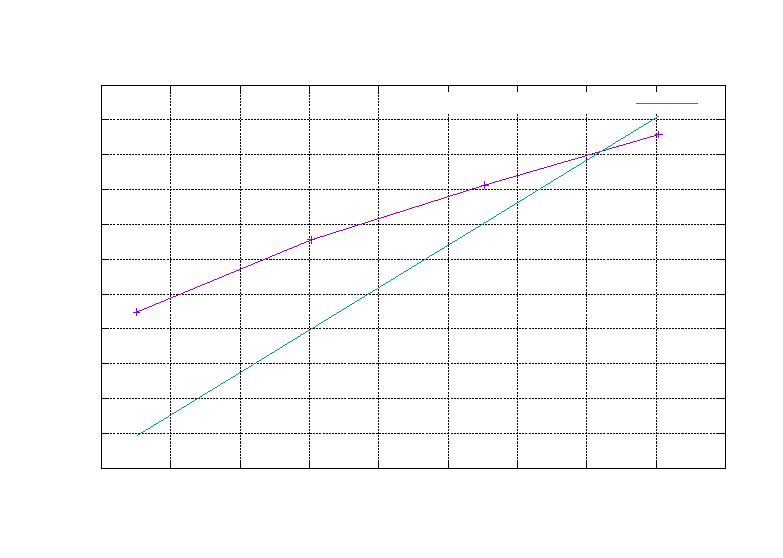
\includegraphics[width={360.00bp},height={252.00bp}]{./Grafy/szeregowo/dynamiczna/graf}}%
    \gplfronttext
  \end{picture}%
\endgroup

    \begin{table}[h!]
        \centering
        \begin{tabular}{|c|c|c|c|}
            \hline
            Masa ciężarków[kg] & \rrtabname & \Ts & stała sprężystości k\\
            \hline
            0.050155 & 9.48 & \pgfmath{(8.54+8.53+8.36)/3/20} & \pgfmathparse{4*(3.14)^2 * 0.050155  / ((8.54+8.53+8.36)/(3*20))^2}\pgfmathresult\\  
            \hline
            0.100478 & 10.55 & \pgfmath{(10.56+10.55+10.55)/3/20} & \pgfmathparse{4*(3.14)^2 * 0.100478  / ((10.56+10.55+10.55)/(3*20))^2}\pgfmathresult\\    
            \hline
            0.150614 & 12.13 & \pgfmath{(12.15+12.13+12.11)/3/20} & \pgfmathparse{4*(3.14)^2 * 0.150614  / ((12.15+12.13+12.11)/(3*20))^2}\pgfmathresult\\    
            \hline
            0.200790 & 13.58 & \pgfmath{(13.58+13.57+13.59)/3/20} & \pgfmathparse{4*(3.14)^2 * 0.200790  / ((13.58+13.57+13.59)/(3*20))^2}\pgfmathresult\\  
            \hline
            \multicolumn{3}{|c|}{\textbf{Średnia}} & \pgfmathparse{((4*(3.14)^2 * 0.050155  / ((8.54+8.53+8.36)/(3*20))^2) + (4*(3.14)^2 * 0.100478  / ((10.56+10.55+10.55)/(3*20))^2) + (4*(3.14)^2 * 0.150614  / ((12.15+12.13+12.11)/(3*20))^2) + (4*(3.14)^2 * 0.200790  / ((13.58+13.57+13.59)/(3*20))^2))/4}\pgfmathresult \\
            \hline
        \end{tabular}
    \end{table} 
    
    \pagebreak
    %niepewność pomiaru
    Niepewność pomiaru wydłużenia sprężyny oszacowaliśmy na 0,1 cm.
    Niepewność pomiaru współczynnika sprężystości:
    \\f(x) = 0.061*x + 1.862 \\
    f'(x) = 0.061 \\
    Średnia wartość współczynnika sprężystości sprężyny:
    \[ k = \pgfmathparse{((4*(3.14)^2 * 0.050155  / ((8.54+8.53+8.36)/(3*20))^2) + (4*(3.14)^2 * 0.100478  / ((10.56+10.55+10.55)/(3*20))^2) + (4*(3.14)^2 * 0.150614  / ((12.15+12.13+12.11)/(3*20))^2) + (4*(3.14)^2 * 0.200790  / ((13.58+13.57+13.59)/(3*20))^2))/4}\pgfmathresult \]
    Zatem: 
    \[ k = (\pgfmathparse{((4*(3.14)^2 * 0.050155  / ((8.54+8.53+8.36)/(3*20))^2) + (4*(3.14)^2 * 0.100478  / ((10.56+10.55+10.55)/(3*20))^2) + (4*(3.14)^2 * 0.150614  / ((12.15+12.13+12.11)/(3*20))^2) + (4*(3.14)^2 * 0.200790  / ((13.58+13.57+13.59)/(3*20))^2))/4}\pgfmathresult \pm  0.061) \frac{N}{m} \]
    Korzystając ze wzoru $k = k_1 + k_2$ możemy obliczyć teoretyczną wartość współczynnika sprężystości.
    \[ k = 10.01283 +  9.547 = \pgfmathparse{10.01283 +  9.547}\pgfmathresult\]
    Wynik mierzony daleki jest teoretycznemu co oznacza mało dokładne, bądź błędne pomiary.\\

    %M7.5
    \textbf{M7.5}
    Wyznaczanie współczynnika sprężystości sprężyn połączonych szeregowo \\
    
    \textbf{a)}
    Metoda statyczna \\
    % GNUPLOT: LaTeX picture with Postscript
\begingroup
  \makeatletter
  \providecommand\color[2][]{%
    \GenericError{(gnuplot) \space\space\space\@spaces}{%
      Package color not loaded in conjunction with
      terminal option `colourtext'%
    }{See the gnuplot documentation for explanation.%
    }{Either use 'blacktext' in gnuplot or load the package
      color.sty in LaTeX.}%
    \renewcommand\color[2][]{}%
  }%
  \providecommand\includegraphics[2][]{%
    \GenericError{(gnuplot) \space\space\space\@spaces}{%
      Package graphicx or graphics not loaded%
    }{See the gnuplot documentation for explanation.%
    }{The gnuplot epslatex terminal needs graphicx.sty or graphics.sty.}%
    \renewcommand\includegraphics[2][]{}%
  }%
  \providecommand\rotatebox[2]{#2}%
  \@ifundefined{ifGPcolor}{%
    \newif\ifGPcolor
    \GPcolorfalse
  }{}%
  \@ifundefined{ifGPblacktext}{%
    \newif\ifGPblacktext
    \GPblacktexttrue
  }{}%
  % define a \g@addto@macro without @ in the name:
  \let\gplgaddtomacro\g@addto@macro
  % define empty templates for all commands taking text:
  \gdef\gplbacktext{}%
  \gdef\gplfronttext{}%
  \makeatother
  \ifGPblacktext
    % no textcolor at all
    \def\colorrgb#1{}%
    \def\colorgray#1{}%
  \else
    % gray or color?
    \ifGPcolor
      \def\colorrgb#1{\color[rgb]{#1}}%
      \def\colorgray#1{\color[gray]{#1}}%
      \expandafter\def\csname LTw\endcsname{\color{white}}%
      \expandafter\def\csname LTb\endcsname{\color{black}}%
      \expandafter\def\csname LTa\endcsname{\color{black}}%
      \expandafter\def\csname LT0\endcsname{\color[rgb]{1,0,0}}%
      \expandafter\def\csname LT1\endcsname{\color[rgb]{0,1,0}}%
      \expandafter\def\csname LT2\endcsname{\color[rgb]{0,0,1}}%
      \expandafter\def\csname LT3\endcsname{\color[rgb]{1,0,1}}%
      \expandafter\def\csname LT4\endcsname{\color[rgb]{0,1,1}}%
      \expandafter\def\csname LT5\endcsname{\color[rgb]{1,1,0}}%
      \expandafter\def\csname LT6\endcsname{\color[rgb]{0,0,0}}%
      \expandafter\def\csname LT7\endcsname{\color[rgb]{1,0.3,0}}%
      \expandafter\def\csname LT8\endcsname{\color[rgb]{0.5,0.5,0.5}}%
    \else
      % gray
      \def\colorrgb#1{\color{black}}%
      \def\colorgray#1{\color[gray]{#1}}%
      \expandafter\def\csname LTw\endcsname{\color{white}}%
      \expandafter\def\csname LTb\endcsname{\color{black}}%
      \expandafter\def\csname LTa\endcsname{\color{black}}%
      \expandafter\def\csname LT0\endcsname{\color{black}}%
      \expandafter\def\csname LT1\endcsname{\color{black}}%
      \expandafter\def\csname LT2\endcsname{\color{black}}%
      \expandafter\def\csname LT3\endcsname{\color{black}}%
      \expandafter\def\csname LT4\endcsname{\color{black}}%
      \expandafter\def\csname LT5\endcsname{\color{black}}%
      \expandafter\def\csname LT6\endcsname{\color{black}}%
      \expandafter\def\csname LT7\endcsname{\color{black}}%
      \expandafter\def\csname LT8\endcsname{\color{black}}%
    \fi
  \fi
    \setlength{\unitlength}{0.0500bp}%
    \ifx\gptboxheight\undefined%
      \newlength{\gptboxheight}%
      \newlength{\gptboxwidth}%
      \newsavebox{\gptboxtext}%
    \fi%
    \setlength{\fboxrule}{0.5pt}%
    \setlength{\fboxsep}{1pt}%
\begin{picture}(7200.00,5040.00)%
    \gplgaddtomacro\gplbacktext{%
      \csname LTb\endcsname%%
      \put(682,704){\makebox(0,0)[r]{\strut{}$-5$}}%
      \csname LTb\endcsname%%
      \put(682,1072){\makebox(0,0)[r]{\strut{}$0$}}%
      \csname LTb\endcsname%%
      \put(682,1439){\makebox(0,0)[r]{\strut{}$5$}}%
      \csname LTb\endcsname%%
      \put(682,1807){\makebox(0,0)[r]{\strut{}$10$}}%
      \csname LTb\endcsname%%
      \put(682,2174){\makebox(0,0)[r]{\strut{}$15$}}%
      \csname LTb\endcsname%%
      \put(682,2542){\makebox(0,0)[r]{\strut{}$20$}}%
      \csname LTb\endcsname%%
      \put(682,2909){\makebox(0,0)[r]{\strut{}$25$}}%
      \csname LTb\endcsname%%
      \put(682,3277){\makebox(0,0)[r]{\strut{}$30$}}%
      \csname LTb\endcsname%%
      \put(682,3644){\makebox(0,0)[r]{\strut{}$35$}}%
      \csname LTb\endcsname%%
      \put(682,4012){\makebox(0,0)[r]{\strut{}$40$}}%
      \csname LTb\endcsname%%
      \put(682,4379){\makebox(0,0)[r]{\strut{}$45$}}%
      \csname LTb\endcsname%%
      \put(814,484){\makebox(0,0){\strut{}$0$}}%
      \csname LTb\endcsname%%
      \put(2012,484){\makebox(0,0){\strut{}$50$}}%
      \csname LTb\endcsname%%
      \put(3210,484){\makebox(0,0){\strut{}$100$}}%
      \csname LTb\endcsname%%
      \put(4407,484){\makebox(0,0){\strut{}$150$}}%
      \csname LTb\endcsname%%
      \put(5605,484){\makebox(0,0){\strut{}$200$}}%
      \csname LTb\endcsname%%
      \put(6803,484){\makebox(0,0){\strut{}$250$}}%
    }%
    \gplgaddtomacro\gplfronttext{%
      \csname LTb\endcsname%%
      \put(209,2541){\rotatebox{-270}{\makebox(0,0){\strut{}Wydłużenie[cm]}}}%
      \put(3808,154){\makebox(0,0){\strut{}Masa ciężarków[g]}}%
      \csname LTb\endcsname%%
      \put(5816,4206){\makebox(0,0)[r]{\strut{}$0.206*x + -0.556$}}%
      \csname LTb\endcsname%%
      \put(3808,4709){\makebox(0,0){\strut{}Otrzymane wyniki za pomocą metody statycznej}}%
    }%
    \gplbacktext
    \put(0,0){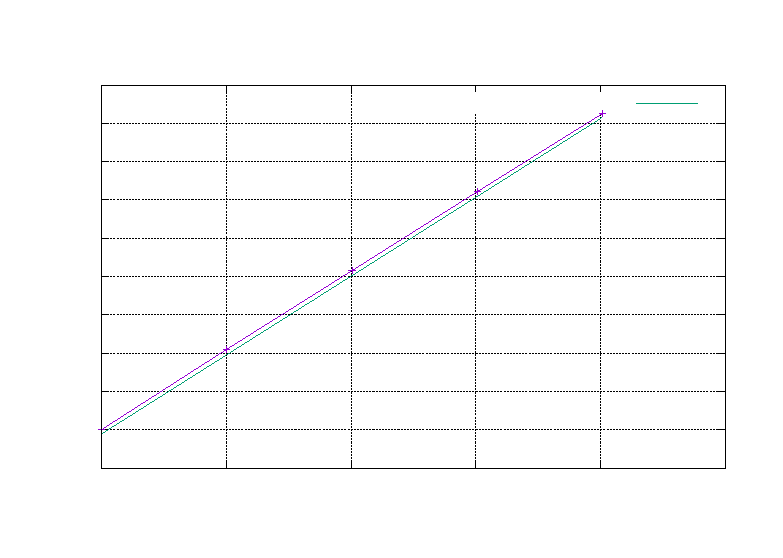
\includegraphics[width={360.00bp},height={252.00bp}]{./Grafy/rownolegle/statyczna/graf}}%
    \gplfronttext
  \end{picture}%
\endgroup

    \pagebreak
    \begin{table}[h!]
        \centering
        \begin{tabular}{|c|c|c|}
            \hline
            Masa ciężarków[kg] & Wydłużenie[m] & stała sprężystości k\\
            \hline
            0.050155  & 0.105 & \pgfmathparse{9.81*0.050155/0.105}\pgfmathresult\\  
            \hline
            0.100478  & 0.208 & \pgfmathparse{9.81*0.100478/0.208}\pgfmathresult\\    
            \hline
            0.150614 & 0.311 & \pgfmathparse{9.81*0.150614/0.311}\pgfmathresult\\    
            \hline
            0.200790 & 0.413 & \pgfmathparse{9.81*0.200790/0.413}\pgfmathresult\\   
            \hline
            \multicolumn{2}{|c|}{\textbf{Średnia}} & \pgfmathparse{(9.81*0.050155/0.105 + 9.81*0.100478/0.208 + 9.81*0.150614/0.311 + 9.81*0.200790/0.413)/4}\pgfmathresult \\
            \hline
        \end{tabular}
        \caption{obliczanie stałej k dla poszczególnych pomiarów.}
    \end{table}
    
    %niepewność pomiaru
    Niepewność pomiaru wydłużenia sprężyny oszacowaliśmy na 0,1 cm.
    Niepewność pomiaru współczynnika sprężystości:
    \\f(x) = 0.206*x + -0.556 \\
    f'(x) = 0.206 \\
    
    Średnia wartość współczynnika sprężystości sprężyny:
    \[ k = \pgfmathparse{(9.81*0.050155/0.105 + 9.81*0.100478/0.208 + 9.81*0.150614/0.311 + 9.81*0.200790/0.413)/4}\pgfmathresult\ \]
    Zatem: 
    \[ k = (\pgfmathparse{(9.81*0.050155/0.105 + 9.81*0.100478/0.208 + 9.81*0.150614/0.311 + 9.81*0.200790/0.413)/4}\pgfmathresult\ \pm  0.206) \frac{N}{m} \]
    Korzystając ze wzoru $\frac{1}{k} = \frac{1}{k_1} + \frac{1}{k_2}$ oraz co za tym idzie $k = \frac{k_1k_2}{k_1+k_2}$ możemy obliczyć teoretyczną wartość współczynnika sprężystości.
    \[ k = \frac{9.85445 * 9.84338}{9.85445 +  9.84338} = \pgfmathparse{(9.85445*9.84338)/(9.85445 +  9.84338)}\pgfmathresult\]
    Wynik mierzony bliski jest temu teoretycznemu. \\
    \pagebreak 
    
    \textbf{b)}
    Metoda dynamiczna \\
    
    % GNUPLOT: LaTeX picture with Postscript
\begingroup
  \makeatletter
  \providecommand\color[2][]{%
    \GenericError{(gnuplot) \space\space\space\@spaces}{%
      Package color not loaded in conjunction with
      terminal option `colourtext'%
    }{See the gnuplot documentation for explanation.%
    }{Either use 'blacktext' in gnuplot or load the package
      color.sty in LaTeX.}%
    \renewcommand\color[2][]{}%
  }%
  \providecommand\includegraphics[2][]{%
    \GenericError{(gnuplot) \space\space\space\@spaces}{%
      Package graphicx or graphics not loaded%
    }{See the gnuplot documentation for explanation.%
    }{The gnuplot epslatex terminal needs graphicx.sty or graphics.sty.}%
    \renewcommand\includegraphics[2][]{}%
  }%
  \providecommand\rotatebox[2]{#2}%
  \@ifundefined{ifGPcolor}{%
    \newif\ifGPcolor
    \GPcolorfalse
  }{}%
  \@ifundefined{ifGPblacktext}{%
    \newif\ifGPblacktext
    \GPblacktexttrue
  }{}%
  % define a \g@addto@macro without @ in the name:
  \let\gplgaddtomacro\g@addto@macro
  % define empty templates for all commands taking text:
  \gdef\gplbacktext{}%
  \gdef\gplfronttext{}%
  \makeatother
  \ifGPblacktext
    % no textcolor at all
    \def\colorrgb#1{}%
    \def\colorgray#1{}%
  \else
    % gray or color?
    \ifGPcolor
      \def\colorrgb#1{\color[rgb]{#1}}%
      \def\colorgray#1{\color[gray]{#1}}%
      \expandafter\def\csname LTw\endcsname{\color{white}}%
      \expandafter\def\csname LTb\endcsname{\color{black}}%
      \expandafter\def\csname LTa\endcsname{\color{black}}%
      \expandafter\def\csname LT0\endcsname{\color[rgb]{1,0,0}}%
      \expandafter\def\csname LT1\endcsname{\color[rgb]{0,1,0}}%
      \expandafter\def\csname LT2\endcsname{\color[rgb]{0,0,1}}%
      \expandafter\def\csname LT3\endcsname{\color[rgb]{1,0,1}}%
      \expandafter\def\csname LT4\endcsname{\color[rgb]{0,1,1}}%
      \expandafter\def\csname LT5\endcsname{\color[rgb]{1,1,0}}%
      \expandafter\def\csname LT6\endcsname{\color[rgb]{0,0,0}}%
      \expandafter\def\csname LT7\endcsname{\color[rgb]{1,0.3,0}}%
      \expandafter\def\csname LT8\endcsname{\color[rgb]{0.5,0.5,0.5}}%
    \else
      % gray
      \def\colorrgb#1{\color{black}}%
      \def\colorgray#1{\color[gray]{#1}}%
      \expandafter\def\csname LTw\endcsname{\color{white}}%
      \expandafter\def\csname LTb\endcsname{\color{black}}%
      \expandafter\def\csname LTa\endcsname{\color{black}}%
      \expandafter\def\csname LT0\endcsname{\color{black}}%
      \expandafter\def\csname LT1\endcsname{\color{black}}%
      \expandafter\def\csname LT2\endcsname{\color{black}}%
      \expandafter\def\csname LT3\endcsname{\color{black}}%
      \expandafter\def\csname LT4\endcsname{\color{black}}%
      \expandafter\def\csname LT5\endcsname{\color{black}}%
      \expandafter\def\csname LT6\endcsname{\color{black}}%
      \expandafter\def\csname LT7\endcsname{\color{black}}%
      \expandafter\def\csname LT8\endcsname{\color{black}}%
    \fi
  \fi
    \setlength{\unitlength}{0.0500bp}%
    \ifx\gptboxheight\undefined%
      \newlength{\gptboxheight}%
      \newlength{\gptboxwidth}%
      \newsavebox{\gptboxtext}%
    \fi%
    \setlength{\fboxrule}{0.5pt}%
    \setlength{\fboxsep}{1pt}%
\begin{picture}(7200.00,5040.00)%
    \gplgaddtomacro\gplbacktext{%
      \csname LTb\endcsname%%
      \put(682,704){\makebox(0,0)[r]{\strut{}$8$}}%
      \csname LTb\endcsname%%
      \put(682,1072){\makebox(0,0)[r]{\strut{}$10$}}%
      \csname LTb\endcsname%%
      \put(682,1439){\makebox(0,0)[r]{\strut{}$12$}}%
      \csname LTb\endcsname%%
      \put(682,1807){\makebox(0,0)[r]{\strut{}$14$}}%
      \csname LTb\endcsname%%
      \put(682,2174){\makebox(0,0)[r]{\strut{}$16$}}%
      \csname LTb\endcsname%%
      \put(682,2542){\makebox(0,0)[r]{\strut{}$18$}}%
      \csname LTb\endcsname%%
      \put(682,2909){\makebox(0,0)[r]{\strut{}$20$}}%
      \csname LTb\endcsname%%
      \put(682,3277){\makebox(0,0)[r]{\strut{}$22$}}%
      \csname LTb\endcsname%%
      \put(682,3644){\makebox(0,0)[r]{\strut{}$24$}}%
      \csname LTb\endcsname%%
      \put(682,4012){\makebox(0,0)[r]{\strut{}$26$}}%
      \csname LTb\endcsname%%
      \put(682,4379){\makebox(0,0)[r]{\strut{}$28$}}%
      \csname LTb\endcsname%%
      \put(814,484){\makebox(0,0){\strut{}$40$}}%
      \csname LTb\endcsname%%
      \put(1479,484){\makebox(0,0){\strut{}$60$}}%
      \csname LTb\endcsname%%
      \put(2145,484){\makebox(0,0){\strut{}$80$}}%
      \csname LTb\endcsname%%
      \put(2810,484){\makebox(0,0){\strut{}$100$}}%
      \csname LTb\endcsname%%
      \put(3476,484){\makebox(0,0){\strut{}$120$}}%
      \csname LTb\endcsname%%
      \put(4141,484){\makebox(0,0){\strut{}$140$}}%
      \csname LTb\endcsname%%
      \put(4807,484){\makebox(0,0){\strut{}$160$}}%
      \csname LTb\endcsname%%
      \put(5472,484){\makebox(0,0){\strut{}$180$}}%
      \csname LTb\endcsname%%
      \put(6138,484){\makebox(0,0){\strut{}$200$}}%
      \csname LTb\endcsname%%
      \put(6803,484){\makebox(0,0){\strut{}$220$}}%
    }%
    \gplgaddtomacro\gplfronttext{%
      \csname LTb\endcsname%%
      \put(209,2541){\rotatebox{-270}{\makebox(0,0){\strut{}Czas wykonywania 20 wachań[s]}}}%
      \put(3808,154){\makebox(0,0){\strut{}Masa ciężarków[g]}}%
      \csname LTb\endcsname%%
      \put(5816,4206){\makebox(0,0)[r]{\strut{}$0.117*x + 3.269$}}%
      \csname LTb\endcsname%%
      \put(3808,4709){\makebox(0,0){\strut{}Otrzymane wyniki za pomocą metody dynamicznej}}%
    }%
    \gplbacktext
    \put(0,0){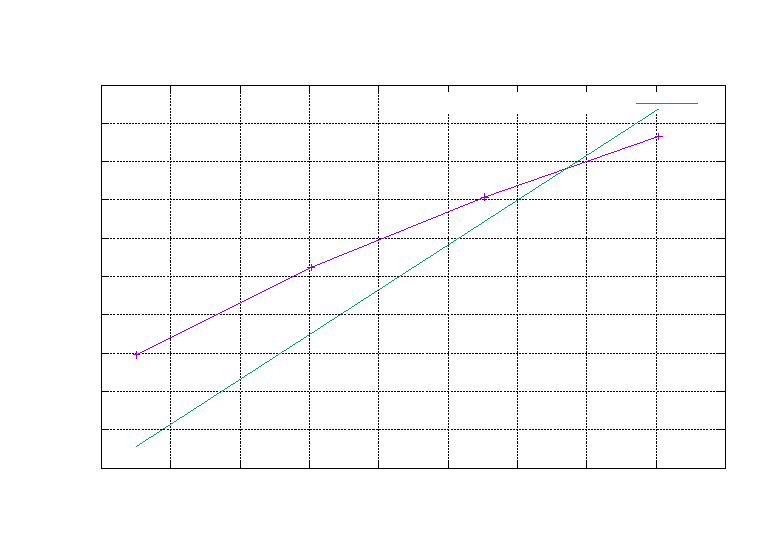
\includegraphics[width={360.00bp},height={252.00bp}]{./Grafy/rownolegle/dynamiczna/graf}}%
    \gplfronttext
  \end{picture}%
\endgroup

    \begin{table}[h!]
        \centering
        \begin{tabular}{|c|c|c|c|}
            \hline
            Masa ciężarków[kg] & \rrtabname & \Ts & stała sprężystości k\\
            \hline
            0.050155 & 13.92 & \pgfmath{(13.91+13.88+13.96)/3/20} & \pgfmathparse{4*(3.14)^2 * 0.050155  / ((13.91+13.88+13.96)/(3*20))^2}\pgfmathresult\\  
            \hline
            0.100478 & 18.48 & \pgfmath{(18.58+18.45+18.40)/3/20} & \pgfmathparse{4*(3.14)^2 * 0.100478  / ((18.58+18.45+18.40)/(3*20))^2}\pgfmathresult\\    
            \hline
            0.150614 & 22.16 & \pgfmath{(22.16+22.15+22.16)/3/20} & \pgfmathparse{4*(3.14)^2 * 0.150614  / ((22.16+22.15+22.16)/(3*20))^2}\pgfmathresult\\    
            \hline
            0.200790 & 25.33 & \pgfmath{(25.32+25.36+25.30)/3/20} & \pgfmathparse{4*(3.14)^2 * 0.200790  / ((25.32+25.36+25.30)/(3*20))^2}\pgfmathresult\\  
            \hline
            \multicolumn{3}{|c|}{\textbf{Średnia}} & \pgfmathparse{((4*(3.14)^2 * 0.050155  / ((13.91+13.88+13.96)/(3*20))^2) + (4*(3.14)^2 * 0.100478  / ((18.58+18.45+18.40)/(3*20))^2) + (4*(3.14)^2 * 0.150614  / ((22.16+22.15+22.16)/(3*20))^2) + (4*(3.14)^2 * 0.200790  / ((25.32+25.36+25.30)/(3*20))^2))/4}\pgfmathresult \\
            \hline
        \end{tabular}
    \end{table}
     
    %niepewność pomiaru
    Niepewność pomiaru wydłużenia sprężyny oszacowaliśmy na 0,1 cm.
    Niepewność pomiaru współczynnika sprężystości:
    \\f(x) = 0.117*x + 3.269 \\
    f'(x) = 0.117 \\
    
    Średnia wartość współczynnika sprężystości sprężyny:
    \[ k = \pgfmathparse{((4*(3.14)^2 * 0.050155  / ((13.91+13.88+13.96)/(3*20))^2) + (4*(3.14)^2 * 0.100478  / ((18.58+18.45+18.40)/(3*20))^2) + (4*(3.14)^2 * 0.150614  / ((22.16+22.15+22.16)/(3*20))^2) + (4*(3.14)^2 * 0.200790  / ((25.32+25.36+25.30)/(3*20))^2))/4}\pgfmathresult \]
    Zatem: 
    \[ k = (\pgfmathparse{((4*(3.14)^2 * 0.050155  / ((13.91+13.88+13.96)/(3*20))^2) + (4*(3.14)^2 * 0.100478  / ((18.58+18.45+18.40)/(3*20))^2) + (4*(3.14)^2 * 0.150614  / ((22.16+22.15+22.16)/(3*20))^2) + (4*(3.14)^2 * 0.200790  / ((25.32+25.36+25.30)/(3*20))^2))/4}\pgfmathresult \pm  0.117) \frac{N}{m} \]
    \pagebreak
    
    Korzystając ze wzoru $\frac{1}{k} = \frac{1}{k_1} + \frac{1}{k_2}$ oraz co za tym idzie $k = \frac{k_1k_2}{k_1+k_2}$ możemy obliczyć teoretyczną wartość współczynnika sprężystości.
    \[ k = \frac{10.01283 * 9.547}{10.01283 +  9.547} = \pgfmathparse{(10.01283*9.547)/(10.01283 +  9.547)}\pgfmathresult\]
    Wynik mierzony bliski jest temu teoretycznemu.
    
    \section{Źródła}
    %kod metody najmniejszych kwadratów.
    Kod użyty znalezienia prostych za pomocą metody najmniejszych kwadratów.
    %chyba usunąć te dolne, zostawić funkcje i 1 przykład
    \begin{minted}{python}
def calculateB(x, y, n):
	sx = sum(x)
	sy = sum(y)
	sxsy = 0
	sx2 = 0

	for i in range(n):
		sxsy += x[i] * y[i]
		sx2 += x[i] * x[i]
	b = (n * sxsy - sx * sy)/(n * sx2 - sx * sx)
	return b

def leastRegLine(X,Y,n):
	b = calculateB(X, Y, n)
	meanX = int(sum(X)/n)
	meanY = int(sum(Y)/n)

	a = meanY - b * meanX

	print("Y = ", '%.3f'%b,"*x + ",'%.3f'%a, sep="")

#pierwsza sprężyna, metoda statyczna
print("pierwsza sprezyna, metoda statyczna:")
X = [0, 50.320, 100.342  , 150.596, 200.861 ]
Y = [0, 5, 10, 15, 20 ]
n = len(X)
leastRegLine(X, Y, n)

#pierwsza sprężyna, metoda dynamiczna
print("pierwsza sprezyna, metoda dynamiczna:")
X = [0, 50.152 , 100.508 , 150.830, 201.095 ]
Y = [0, (9.31+9.21+9.23)/3, (12.59+12.68+12.56)/3, (15.25+15.17+15.16)/3, (17.40+17.41+17.28)/3 ]
n = len(X)
leastRegLine(X, Y, n)

#druga sprężyna, metoda statyczna
print("druga sprezyna, metoda statyczna:")
X = [0, 50.155 , 100.478 , 150.614, 200.790 ]
Y = [0, 4.8, 10, 15.3, 20.5 ]
n = len(X)
leastRegLine(X, Y, n)

#druga sprężyna, metoda dynamiczna
print("druga sprezyna, metoda dynamiczna:")
X = [0, 50.155, 100.478 , 150.614, 200.790 ]
Y = [0, (9.53+9.49)/2, (12.89+12.93)/2, (15.57+15.43)/2, (17.76+17.77)/2 ]
n = len(X)
leastRegLine(X, Y, n)

#szeregowo sprężyny, metoda statyczna
print("szeregowo sprezyny, metoda statyczna:")
X = [0, 50.155, 100.478 , 150.614, 200.790 ]
Y = [0, 2.5, 5.2, 7.8, 10.2 ]
n = len(X)
leastRegLine(X, Y, n)

#szeregowo sprężyny, metoda dynamiczna
print("szeregowo sprezyny, metoda dynamiczna:")
X = [0, 50.155, 100.478 , 150.614, 200.790 ]
Y = [0, (8.54+8.53+8.36)/3, (10.56+10.55+10.55)/3, (12.15+12.13+12.11)/3, (13.58+13.57+13.59)/3 ]
n = len(X)
leastRegLine(X, Y, n)

#rownolegle sprężyny, metoda statyczna
print("rownolegle sprezyny, metoda statyczna:")
X = [0, 50.155, 100.478 , 150.614, 200.790 ]
Y = [0, 10.5, 20.8, 31.1, 41.3 ]
n = len(X)
leastRegLine(X, Y, n)

#rownolegle sprężyny, metoda dynamiczna
print("rownolegle sprezyny, metoda dynamiczna:")
X = [0, 50.155, 100.478 , 150.614, 200.790 ]
Y = [0, (13.91+13.88+13.96)/3, (18.58+18.45+18.40)/3, (22.16+22.15+22.16)/3, (25.32+25.36+25.30)/3 ]
n = len(X)
leastRegLine(X, Y, n)

    \end{minted}

\end{document}